\chapter[Leçon 40: Sech virstellen, Famill, Aarbecht, Sproochen \& Liesen]{Leçon 40: Sech virstellen, Famill a Geschwëster, Aarbecht, Sproochen \& Bicher liesen}

Dës Lektioun verbënnt déi wichtegst kommunikativ Grondstrukture fir den Alldag mat zentrale Konversatiouns- a Sproochentest-Themen. Am éischten Deel léiere mir, wéi ee \textbf{sech selwer a seng Famill virstellt} (Numm, Familljennumm, Alter, Wunnuert, Joreszuelen, Kanner a Geschwëster), mat engem besonnesche Fokus op den Ënnerscheed tëscht \textbf{zwee / zwéin} an der femininner Form \textbf{zwou}, de Gebrauch vun de \textbf{Besëtzpronomen} (\textit{mäin/mäi/meng}, \textit{däin/däi/deng}) an d'Vermeidung vu Verwiesslungen tëscht \textbf{d'Schwëster} (la sœur / the sister) a \textbf{schwätzen} (parler / to speak). Am zweeten Deel behandele mir den \textbf{Uerts- a Sazbau} (\textit{hei}, \textit{hei am Land}, \textit{do}, \textit{doheem} vs. \textit{vun doheem}, d'Inversioun vum Verb no enger Uertsbestëmmung, d'Froewuert \textbf{firwat} mat der Konjunktioun \textbf{well} an d'Prepositiounen \textbf{zënter / zanter / säit}). Duerno geet et ëm \textbf{Beruff, Aarbecht, Landwirtschaft a Sproochen} (d'Verben \textit{heeschen}, \textit{schaffen}, \textit{planzen}, \textit{kafen}, \textit{schwätzen} a \textit{kënnen}), ier mir d'Lektioun mat engem Thema fir Fortgeschrattener ofschléissen : \textbf{Bicher a Liesegewunnechten} (\textit{d'Geschicht} vs. \textit{d'Gesiicht}, \textit{spannend}, \textit{Et geet ëm...}).

\textit{Cette leçon relie les structures communicatives fondamentales du quotidien aux grands thèmes de conversation et du \textbf{Sproochentest}. Dans la première partie, nous apprenons à \textbf{se présenter et présenter sa famille} (prénom, nom de famille, âge, lieu de résidence, années, enfants et frères et sœurs), en insistant sur l'accord du chiffre deux (\textbf{zwee / zwéin} vs le féminin obligatoire \textbf{zwou}), l'emploi des \textbf{adjectifs possessifs} (\textit{mäin/mäi/meng}, \textit{däin/däi/deng}) et la distinction essentielle entre \textbf{d'Schwëster} (la sœur) et le verbe \textbf{schwätzen} (parler). Dans la deuxième partie, nous étudions les \textbf{adverbes de lieu et l'ordre des mots} (\textit{hei}, \textit{hei am Land}, \textit{do}, \textit{doheem} vs \textit{vun doheem}, l'inversion sujet-verbe, la question \textbf{firwat} avec \textbf{well}, ainsi que les prépositions de durée \textbf{zënter / zanter / säit}). Nous abordons ensuite \textbf{le travail, les professions, l'agriculture et les langues parlées} (conjugaison de \textit{heeschen}, \textit{schaffen}, \textit{planzen}, \textit{kafen}, \textit{schwätzen} et \textit{kënnen}), avant de conclure par un volet consacré aux \textbf{livres et habitudes de lecture} (\textit{d'Geschicht} vs \textit{d'Gesiicht}, \textit{spannend}, \textit{Et geet ëm...}).}

\textit{This lesson connects essential everyday communicative structures with core conversation and \textbf{Sproochentest} topics. In the first part, we learn how to \textbf{introduce oneself and one's family} (first name, surname, age, place of residence, years, children, and siblings), with special attention to gender agreement for the number two (\textbf{zwee / zwéin} vs. the mandatory feminine \textbf{zwou}), \textbf{possessive adjectives} (\textit{mäin/mäi/meng}, \textit{däin/däi/deng}), and avoiding confusion between \textbf{d'Schwëster} (sister) and the verb \textbf{schwätzen} (to speak). In the second part, we cover \textbf{adverbs of place and word order} (\textit{hei}, \textit{hei am Land}, \textit{do}, \textit{doheem} vs. \textit{vun doheem}, subject-verb inversion, asking \textbf{firwat} and answering with \textbf{well}, and the duration prepositions \textbf{zënter / zanter / säit}). Next, we explore \textbf{work, professions, agriculture, and spoken languages} (conjugating \textit{heeschen}, \textit{schaffen}, \textit{planzen}, \textit{kafen}, \textit{schwätzen}, and \textit{kënnen}), and finish with an advanced section on \textbf{books and reading habits} (\textit{d'Geschicht} vs. \textit{d'Gesiicht}, \textit{spannend}, \textit{Et geet ëm...}).}

\vspace{1.5em}

% ==============================================================================
% SECTION I: SECH VIRSTELLEN, ZUELEN, JOREN A KANNER
% ==============================================================================
\section[Sech virstellen, Zuelen, Joren a Kanner / Self-Introduction, Numbers and Children]{Sech virstellen, Zuelen, Joren a Kanner \\/ Se présenter, les nombres, les années et les enfants \\/ Self-Introduction, Numbers, Years and Children}

\subsection{Sech kuerz virstellen : Numm, Alter a Wunnuert / Se présenter brièvement / Brief Self-Introduction}

Wann ee sech op Lëtzebuergesch virstellt, kombinéiert een d'Verben \textbf{sinn} (être / to be), \textbf{heeschen} (s'appeler / to be called) a \textbf{wunnen} (habiter / to live) : \\
\textit{FR : Lorsqu'on se présente en luxembourgeois, on combine les verbes \textbf{sinn}, \textbf{heeschen} et \textbf{wunnen} :} \\
\textit{EN : When introducing oneself in Luxembourgish, one combines the verbs \textbf{sinn}, \textbf{heeschen}, and \textbf{wunnen}:}

\begin{itemize}
    \item \textbf{Beispill 1 :} \\
    \textit{Moien ! Wéi geet et ? -- Gutt, Merci ! Ech sinn de Mohammed (oder : Ech heesche Mohammed). Ech sinn eenandrësseg (31) Joer al. Ech wunnen zënter 2022 (zweedausendzweeanzwanzeg) zu Lëtzebuerg, zu Gonnereng (Gonderange).} \\
    $\rightarrow$ \textit{FR :} Bonjour ! Comment ça va ? -- Bien, merci ! Je suis Mohammed (ou : Je m'appelle Mohammed). J'ai trente et un (31) ans. J'habite depuis 2022 au Luxembourg, à Gonderange. \\
    $\rightarrow$ \textit{EN :} Hello! How are you? -- Good, thank you! I am Mohammed (or: My name is Mohammed). I am thirty-one (31) years old. I have been living in Luxembourg, in Gonderange, since 2022.

    \vspace{0.3em}

    \item \textbf{Beispill 2 :} \\
    \textit{Moien ! Ech sinn d'Martina (oder : Mäin Numm ass Martina). Ech kommen aus Italien, vu Genua, an ech wunnen elo hei zu Lëtzebuerg.} \\
    $\rightarrow$ \textit{FR :} Bonjour ! Je suis Martina (ou : Mon nom est Martina). Je viens d'Italie, de Gênes, et j'habite maintenant ici au Luxembourg. \\
    $\rightarrow$ \textit{EN :} Hello! I am Martina (or: My name is Martina). I come from Italy, from Genoa, and I now live here in Luxembourg.

    \vspace{0.3em}

    \item \textbf{Grammatesch Notiz zum Artikel virum Virnumm :} \\
    Op Lëtzebuergesch setzt ee virun e Virnumm meeschtens de bestëmmten Artikel : \textbf{de / den} fir e männleche Virnumm (\textit{Ech sinn \textbf{de} Mohammed / \textbf{den} Andrea}) an \textbf{d'} fir e weibleche Virnumm (\textit{Ech sinn \textbf{d'}Martina / \textbf{d'}Ala}). No dem Verb \textbf{heesche} steet awer \textbf{keen Artikel} (\textit{Ech heesche Mohammed / Meng Fra heescht Ala}). \\
    $\rightarrow$ \textit{FR :} En luxembourgeois, on place généralement l'article défini devant un prénom (\textbf{de/den} pour un homme, \textbf{d'} pour une femme) après \textit{sinn}, mais \textbf{sans article} après le verbe \textit{heeschen}. \\
    $\rightarrow$ \textit{EN :} In Luxembourgish, the definite article (\textbf{de/den} for men, \textbf{d'} for women) is normally used before a first name after \textit{sinn}, whereas \textbf{no article} is used after the verb \textit{heeschen}.
\end{itemize}

\subsection{D'Zuele vun 0 bis 12 an d'Aussprooch vun \textit{ei} vs. \textit{äi} vs. \textit{é / éi} \\/ Les nombres de 0 à 12 et la prononciation de \textit{ei}, \textit{äi} et \textit{é / éi} \\/ Numbers from 0 to 12 and Pronunciation of \textit{ei}, \textit{äi} and \textit{é / éi}}

\begin{table}[htbp]
    \centering
    \small
    \begin{tabular}{cl cl cl}
        \toprule
        \textbf{Zuel} & \textbf{Lëtzebuergesch} & \textbf{Zuel} & \textbf{Lëtzebuergesch} & \textbf{Zuel} & \textbf{Lëtzebuergesch} \\
        \midrule
        \textbf{0} & null & \textbf{5} & fënnef & \textbf{9} & néng {[neŋ]} \\
        \textbf{1} & een / ee (m., n.), eng (f.) & \textbf{6} & sechs & \textbf{10} & zéng {[tseŋ]} \\
        \textbf{2} & zwee (n./m.), zwéin (m.), \textbf{zwou} (f.) & \textbf{7} & siwen & \textbf{11} & eelef \\
        \textbf{3} & dräi {[dʀæːɪ]} & \textbf{8} & aacht & \textbf{12} & zwielef \\
        \textbf{4} & véier {[fəɪɐ]} & & & \textbf{60} & sechsteg \\
        \bottomrule
    \end{tabular}
    \caption{D'Zuele vun 0 bis 12 (an 60) op Lëtzebuergesch (Les nombres / Numbers)}
\end{table}

\begin{itemize}
    \item \textbf{Phoneteschen Tipp : D'Aussprooch vun \textit{ei} {[ɑɪ]} vs. \textit{äi} {[æːɪ]} vs. \textit{é / éi} {[e / ɜɪ]} \\
    / Conseil phonétique : La prononciation de \textit{ei}, \textit{äi} et \textit{é / éi} \\
    / Phonetic Tip: The Pronunciation of \textit{ei}, \textit{äi} and \textit{é / éi}}
    \begin{itemize}
        \item \textbf{ei {[ɑɪ]} -- méi hanneren/zentralen oppenen Ufanksvokal :} \\
        D'Diphthong \textbf{ei} gëtt mat engem hënneschten/zentralen oppene Vokal \textbf{{[ɑɪ]}} ausgeschwat (wéi am däitsche Wuert \textit{mein} oder am englesche \textit{my} / \textit{eye}) : \\
        $\bullet$ \textbf{hei} {[hɑɪ]} (\textit{ici / here}), \textbf{Feier} {[ˈfɑɪɐ]} (\textit{feu / fire}), \textbf{nei} {[nɑɪ]} (\textit{nouveau / new}), \textbf{Leit} {[lɑɪt]} (\textit{gens / people}), \textbf{bleiwen} {[ˈblɑɪvən]} (\textit{rester / to stay}). \\
        $\rightarrow$ \textit{FR : La diphtongue \textbf{ei} se prononce \textbf{[ɑɪ]} (le premier élément est un « a » central/postérieur ouvert, comme dans l'allemand \textit{mein} ou l'anglais \textit{my}) : \textit{hei} (ici), \textit{Feier} (feu), \textit{nei} (nouveau), \textit{Leit} (gens).} \\
        $\rightarrow$ \textit{EN : The diphthong \textbf{ei} is pronounced \textbf{[ɑɪ]} (starting with a central/back open vowel, like German \textit{mein} or English \textit{my} / \textit{eye}): \textit{hei} (here), \textit{Feier} (fire), \textit{nei} (new), \textit{Leit} (people).}

        \vspace{0.3em}

        \item \textbf{äi {[æːɪ]} -- laangen, virwëtzen oppenen Ufanksvokal :} \\
        D'Diphthong \textbf{äi} huet eng aner, däitlech méi hell an no vir gezunne Qualitéit : si fänkt mam laangen, oppene virwëtzege Vokal \textbf{{[æː]}} un (wéi de kuerzen \textit{ä} oder dat englescht \textit{a} a \textit{cat} / \textit{bad}, mee gedehnt a Richtung \textit{i}) : \\
        $\bullet$ \textbf{dräi} {[dʀæːɪ]} (\textit{trois / three}), \textbf{mäin} {[mæːɪn]} (\textit{mon / my}), \textbf{däin} {[dæːɪn]} (\textit{ton / your}), \textbf{säit} {[zæːɪt]} (\textit{depuis / since}), \textbf{Schwäin} {[ʃvæːɪn]} (\textit{cochon / pig}), \textbf{Zäit} {[tsæːɪt]} (\textit{temps / time}). \\
        $\rightarrow$ \textit{FR : La diphtongue \textbf{äi} a une prononciation différente de \textit{ei} : elle commence par une voyelle antérieure très ouverte et allongée \textbf{[æːɪ]} (comme le « a » anglais dans \textit{cat} ou \textit{bad}, plus ouvert et plus antérieur que pour \textit{ei}) : \textit{dräi} (trois), \textit{mäin} (mon), \textit{däin} (ton), \textit{säit} (depuis), \textit{Zäit} (temps).} \\
        $\rightarrow$ \textit{EN : The diphthong \textbf{äi} has a distinct pronunciation from \textit{ei}: it begins with a lengthened, open front vowel \textbf{[æːɪ]} (similar to the vowel in English \textit{cat} or \textit{bad}, held longer and gliding toward \textit{i}, noticeably more front and open than \textit{ei}): \textit{dräi} (three), \textit{mäin} (my), \textit{däin} (your), \textit{säit} (since), \textit{Zäit} (time).}

        \vspace{0.3em}

        \item \textbf{é / éi {[e / ɜɪ]} -- zouene Vokal oder zentréierenden Diphthong :} \\
        D'Buschtawen \textbf{é} (virun \textit{-ng}) an \textbf{éi} dogéint gi vill méi zou wéi \textbf{{[e]}} oder \textbf{{[ɜɪ]}} ausgeschwat : \\
        $\bullet$ \textbf{wéi} {[vɜɪ]} (\textit{comment / how}), \textbf{véier} {[fəɪɐ]} (\textit{quatre / four}), \textbf{néng} {[neŋ]} (\textit{neuf / nine}), \textbf{zéng} {[tseŋ]} (\textit{dix / ten}). \\
        $\rightarrow$ \textit{FR : La voyelle \textbf{é} (devant \textit{-ng}) et la diphtongue \textbf{éi} sont beaucoup plus fermées \textbf{[e]} / \textbf{[ɜɪ]} : \textit{wéi} (comment), \textit{véier} (quatre), \textit{néng} (neuf), \textit{zéng} (dix -- attention à ne pas prononcer comme le mot français « dix » !).} \\
        $\rightarrow$ \textit{EN : The vowel \textbf{é} (before \textit{-ng}) and diphthong \textbf{éi} are much more closed \textbf{[e]} / \textbf{[ɜɪ]}: \textit{wéi} (how), \textit{véier} (four), \textit{néng} (nine), \textit{zéng} (ten -- do not pronounce like the French word \textit{dix}!).}
    \end{itemize}
\end{itemize}

\subsection{Kanner, Genus an d'Zuel \flqq Zwee\frqq{} (\textit{zwee / zwéin} vs. \textit{zwou}) \\/ Les enfants, le genre grammatical et le chiffre « deux » \\/ Children, Grammatical Gender and the Number "Two"}

\begin{itemize}
    \item \textbf{D'Substantiver ronderëm d'Kanner (Les enfants / Children) :}
    \begin{table}[htbp]
        \centering
        \small
        \begin{tabular}{llll}
            \toprule
            \textbf{Singulier} & \textbf{Genus} & \textbf{Pluriel} & \textbf{Iwwersetzung (FR / EN)} \\
            \midrule
            \textbf{e Kand / d'Kand} & Neutrum (\textit{n.}) & \textbf{d'Kanner} & un enfant / a child \\
            \textbf{e Jong / de Jong} & Maskulinum (\textit{m.}) & \textbf{d'Jongen} & un garçon / a boy \\
            \textbf{e Meedchen / d'Meedchen} & \textbf{Neutrum (\textit{n.}) !} & \textbf{d'Meedercher} & une fille / a girl \\
            \bottomrule
        \end{tabular}
        \caption{Kand, Jong a Meedchen : Genus a Pluriel}
    \end{table}

    \item \textbf{Wichteg Grammaire-Regel : D'Zuel 2 passt sech dem Genus un ! \\
    / Règle grammaticale : Le chiffre 2 s'accorde selon le genre ! \\
    / Grammar Rule: The number 2 agrees with grammatical gender!} \\
    Am Lëtzebuergeschen ännert sech d'Zuel \textbf{2} jee no dem grammatesche Geschlecht vum Substantiv (och wann d'Substantiv am Pluriel steet !) : \\
    \textit{FR : En luxembourgeois, le chiffre 2 change de forme selon le genre grammatical du nom qui suit (même lorsque le nom est au pluriel) :} \\
    \textit{EN : In Luxembourgish, the number 2 changes form according to the grammatical gender of the following noun (even when the noun is plural):}
    \begin{enumerate}
        \item \textbf{Neutrum (an ëmgangssproochlech Maskulinum)} $\rightarrow$ \textbf{zwee} (traditionell Maskulinum : \textbf{zwéin}) : \\
        \textit{FR : Neutre (et couramment masculin) $\rightarrow$ \textbf{zwee} (forme masculine traditionnelle : \textbf{zwéin}) :} \\
        \textit{EN : Neuter (and colloquially masculine) $\rightarrow$ \textbf{zwee} (traditional masculine form: \textbf{zwéin}):}
        \begin{itemize}
            \item \textit{Ech hunn \textbf{zwee Kanner}.} (\textit{d'Kand} ass Neutrum) \\
            $\rightarrow$ \textit{FR :} J'ai deux enfants. (\textit{d'Kand} est neutre) \\
            $\rightarrow$ \textit{EN :} I have two children. (\textit{d'Kand} is neuter)
            \item \textit{Ech hunn \textbf{zwee Jongen} (oder : \textbf{zwéi Jongen}).} (\textit{de Jong} ass Maskulinum) \\
            $\rightarrow$ \textit{FR :} J'ai deux garçons. (\textit{de Jong} est masculin) \\
            $\rightarrow$ \textit{EN :} I have two boys. (\textit{de Jong} is masculine)
            \item \textit{Ech hunn \textbf{zwee Meedercher}.} \\
            \textit{(Opgepasst : Well \textit{d'Meedchen} wéinst dem Diminutiv-Suffix \textit{-chen} \textbf{Neutrum} ass, seet een \textbf{zwee Meedercher}, net \textit{*zwou Meedercher} !)} \\
            $\rightarrow$ \textit{FR :} J'ai deux filles. (Attention : \textit{d'Meedchen} étant neutre en raison du suffixe diminutif \textit{-chen}, on dit \textbf{zwee Meedercher}, et non pas \textit{*zwou Meedercher} !) \\
            $\rightarrow$ \textit{EN :} I have two girls. (Note: Because \textit{d'Meedchen} is neuter due to the diminutive suffix \textit{-chen}, one says \textbf{zwee Meedercher}, not \textit{*zwou Meedercher}!)
            \item \textit{Mir hunn \textbf{zwee Hënn} an \textbf{zwee Autoen}.} (\textit{den Hond} an \textit{den Auto} si Maskulinum) \\
            $\rightarrow$ \textit{FR :} Nous avons deux chiens et deux voitures. (\textit{den Hond} et \textit{den Auto} sont masculins) \\
            $\rightarrow$ \textit{EN :} We have two dogs and two cars. (\textit{den Hond} and \textit{den Auto} are masculine)
        \end{itemize}

        \vspace{0.3em}

        \item \textbf{Femininum (obligatoresch !)} $\rightarrow$ \textbf{zwou} : \\
        \textit{FR : Féminin (obligatoire !) $\rightarrow$ \textbf{zwou} :} \\
        \textit{EN : Feminine (mandatory!) $\rightarrow$ \textbf{zwou}:}
        \begin{itemize}
            \item \textit{Si huet \textbf{zwou Kazen}.} (\textit{d'Kaz} ass Femininum $\rightarrow$ Pl. \textit{d'Kazen}) \\
            $\rightarrow$ \textit{FR :} Elle a deux chats. (\textit{d'Kaz} est féminin $\rightarrow$ Pl. \textit{d'Kazen}) \\
            $\rightarrow$ \textit{EN :} She has two cats. (\textit{d'Kaz} is feminine $\rightarrow$ Pl. \textit{d'Kazen})
            \item \textit{Hien huet \textbf{zwou Schwësteren}.} (\textit{d'Schwëster} ass Femininum $\rightarrow$ Pl. \textit{d'Schwësteren}) \\
            $\rightarrow$ \textit{FR :} Il a deux sœurs. (\textit{d'Schwëster} est féminin $\rightarrow$ Pl. \textit{d'Schwësteren}) \\
            $\rightarrow$ \textit{EN :} He has two sisters. (\textit{d'Schwëster} is feminine $\rightarrow$ Pl. \textit{d'Schwësteren})
            \item \textit{Do sinn \textbf{zwou Fraen} an \textbf{zwou Blummen}.} (\textit{d'Fra} an \textit{d'Blumm} si Femininum) \\
            $\rightarrow$ \textit{FR :} Il y a là-bas deux femmes et deux fleurs. (\textit{d'Fra} et \textit{d'Blumm} sont féminins) \\
            $\rightarrow$ \textit{EN :} There are two women and two flowers over there. (\textit{d'Fra} and \textit{d'Blumm} are feminine)
        \end{itemize}
    \end{enumerate}

    \vspace{0.3em}

    \item \textbf{Dialog-Beispiller iwwer d'Kanner an hiren Alter :}
    \begin{itemize}
        \item \textit{Hues du Kanner ? -- Jo, ech hunn \textbf{dräi Kanner} : \textbf{ee Jong}, zéng Joer al, an \textbf{zwee Meedercher}, zwielef an aacht Joer al.} \\
        $\rightarrow$ \textit{FR :} As-tu des enfants ? -- Oui, j'ai trois enfants : un garçon de dix ans et deux filles de douze et huit ans. \\
        $\rightarrow$ \textit{EN :} Do you have children? -- Yes, I have three children: one boy, ten years old, and two girls, twelve and eight years old.
        \item \textit{Hues du Kanner ? -- Nee, ech hu \textbf{keng Kanner}.} \\
        $\rightarrow$ \textit{FR :} As-tu des enfants ? -- Non, je n'ai pas d'enfants. \\
        $\rightarrow$ \textit{EN :} Do you have children? -- No, I do not have any children.
    \end{itemize}
\end{itemize}

\vspace{1.5em}

% ==============================================================================
% SECTION II: FAMILL, GESCHWËSTER, HAUSDÉIEREN A BESËTZPRONOMEN
% ==============================================================================
\section[Famill, Geschwëster a Besëtzpronomen]{Famill, Geschwëster, Hausdéieren a Besëtzpronomen \\/ Famille, frères et sœurs, animaux et adjectifs possessifs \\/ Family, Siblings, Pets and Possessive Adjectives}

\subsection{Nom Numm froen : \textit{heeschen}, \textit{de Virnumm} an \textit{de Familljennumm}}

Et gëtt zwou Haaptmanéiere fir nom Numm vun enger Persoun ze froen : \\
\textit{FR : Il existe deux façons principales de demander le nom d'une personne :} \\
\textit{EN : There are two main ways to ask for someone's name:}

\begin{enumerate}
    \item \textbf{Mam Verb \textit{heeschen} (s'appeler / to be called) :}
    \begin{itemize}
        \item \textit{1. / 2. Persoun Singulier :} \textbf{Wéi heeschs du ?} (informell) / \textbf{Wéi heescht Dir ?} (formell) \\
        $\rightarrow$ \textbf{Ech heesche Mohammed.} / \textbf{Ech heesche Martina.} \\
        $\rightarrow$ \textit{FR :} Comment t'appelles-tu ? / Comment vous appelez-vous ? -- Je m'appelle Mohammed / Martina. \\
        $\rightarrow$ \textit{EN :} What is your name (lit. How are you called)? -- My name is Mohammed / Martina.
        \item \textit{3. Persoun Singulier (\textbf{heescht}) :} \\
        $\bullet$ \textbf{Wéi heescht deng Fra ?} -- \textbf{Meng Fra heescht Ala.} (\textit{FR :} Comment s'appelle ta femme ? -- Ma femme s'appelle Ala. / \textit{EN :} What is your wife's name? -- My wife's name is Ala.) \\
        $\bullet$ \textbf{Wéi heescht däi Mann ?} -- \textbf{Mäi Mann heescht Andrea.} (\textit{FR :} Comment s'appelle ton mari ? -- Mon mari s'appelle Andrea. / \textit{EN :} What is your husband's name? -- My husband's name is Andrea.) \\
        $\bullet$ \textbf{Wéi heescht deng Schwëster ?} -- \textbf{Meng Schwëster heescht Iman.} (\textit{FR :} Comment s'appelle ta sœur ? -- Ma sœur s'appelle Iman. / \textit{EN :} What is your sister's name? -- My sister's name is Iman.)
        \item \textit{3. Persoun Pluriel (\textbf{heeschen}) :} \\
        $\bullet$ \textbf{Wéi heeschen deng Geschwëster / deng Bridder ?} \\
        -- \textbf{Meng Bridder heesche Mostafa, Ahmad, Khaled, Al-Hassan an Ibrahim.} \\
        $\rightarrow$ \textit{FR :} Comment s'appellent tes frères et sœurs / tes frères ? -- Mes frères s'appellent Mostafa, Ahmad, Khaled, Al-Hassan et Ibrahim. \\
        $\rightarrow$ \textit{EN :} What are your siblings' / your brothers' names? -- My brothers are called Mostafa, Ahmad, Khaled, Al-Hassan, and Ibrahim.
    \end{itemize}

    \vspace{0.3em}

    \item \textbf{Mam Substantiv \textit{den Numm} (m.), \textit{de Virnumm} (m.) oder \textit{de Familljennumm} (m., Pl. \textit{d'Familljennimm}) :}
    \begin{itemize}
        \item \textbf{Wat ass däin Numm ?} (oder : \textbf{Wat ass Ären Numm ?}) $\rightarrow$ \textbf{Mäin Numm ass...} \\
        \textit{(Opgepasst : Virum Buschtaf \textbf{N} vun \textit{Numm} bleift den \textbf{-n} vu \textit{mäin / däin / Ären} no der Eifeler Regel stoen !)} \\
        $\rightarrow$ \textit{FR :} Quel est ton / votre nom ? -- Mon nom est... \\
        $\rightarrow$ \textit{EN :} What is your name? -- My name is...
        \item \textbf{Wat ass däi Virnumm a wat ass däi Familljennumm ?} \\
        $\rightarrow$ \textbf{Mäi Virnumm ass Mohammed a mäi Familljennumm ass...} \\
        \textit{(Virum \textbf{V} vu \textit{Virnumm} an dem \textbf{F} vu \textit{Familljennumm} fält den \textbf{-n} ewech : \textbf{mäi / däi / Äre} !)} \\
        $\rightarrow$ \textit{FR :} Quel est ton prénom et quel est ton nom de famille ? -- Mon prénom est Mohammed et mon nom de famille est... \\
        $\rightarrow$ \textit{EN :} What is your first name and what is your surname / last name? -- My first name is Mohammed and my last name is...
    \end{itemize}
\end{enumerate}

\subsection{D'Besëtzpronomen (\textit{mäin/meng}, \textit{däin/deng}, \textit{Ären/Är}) am Iwwerbléck}

Genau wéi den onbestëmmten Artikel (\textit{en/e} vs. \textit{eng}) an d'Negatioun (\textit{keen/kee} vs. \textit{keng}) passe sech och d'Besëtzpronomen (Adjectifs possessifs / Possessive adjectives) dem Genus an der Zuel vum Substantiv un : \\
\textit{FR : Tout comme l'article indéfini et la négation, les adjectifs possessifs s'accordent en genre et en nombre avec le nom possédé :} \\
\textit{EN : Just like the indefinite article and negation, possessive adjectives agree in gender and number with the possessed noun:}

\begin{table}[htbp]
    \centering
    \small
    \begin{tabular}{lllll}
        \toprule
        \textbf{Persoun} & \textbf{Mask. (\textit{m.})} & \textbf{Neutr. (\textit{n.})} & \textbf{Fem. (\textit{f.})} & \textbf{Pluriel (\textit{pl.})} \\
        \midrule
        \textbf{ech} (\textit{mon, ma, mes / my}) & \textbf{mäin} (\textbf{mäi}*) & \textbf{mäin} (\textbf{mäi}*) & \textbf{meng} & \textbf{meng} \\
        \textbf{du} (\textit{ton, ta, tes / your}) & \textbf{däin} (\textbf{däi}*) & \textbf{däin} (\textbf{däi}*) & \textbf{deng} & \textbf{deng} \\
        \textbf{hien / et} (\textit{son, sa, ses / his, its}) & \textbf{säin} (\textbf{säi}*) & \textbf{säin} (\textbf{säi}*) & \textbf{seng} & \textbf{seng} \\
        \textbf{hatt / si} (\textit{son, sa, leur / her, their}) & \textbf{hiren} (\textbf{hire}*) & \textbf{hiert} & \textbf{hir} & \textbf{hir} \\
        \textbf{Dir} (\textit{votre, vos / your [form.]}) & \textbf{Ären} (\textbf{Äre}*) & \textbf{Äert} & \textbf{Är} & \textbf{Är} \\
        \bottomrule
    \end{tabular}
    \caption{D'Besëtzpronomen am Nominativ / Akkusativ (*ouni \textit{-n} no der Eifeler Regel viru Konsonanten ausser \textit{n, d, t, z, h})}
\end{table}

\begin{itemize}
    \item \textbf{Konkret Beispiller mat der Eifeler Regel \\
    / Exemples concrets avec la règle de l'Eifel \\
    / Concrete Examples with the Eifeler Regel :}
    \begin{itemize}
        \item \textbf{Maskulinum :} \textit{mäin Numm, däin Hond, mäin Auto} (virun \textit{N, H, Vokal}) vs. \textit{\textbf{mäi} Mann, \textbf{däi} Familljennumm, \textbf{mäi} Brudder, \textbf{däi} Jong} (viru \textit{M, F, B, J}). \\
        $\rightarrow$ \textit{FR : Masculin : \textbf{-n} maintenu devant n, h, voyelle (\textit{mäin Numm, däin Hond, mäin Auto}) ; \textbf{-n} supprimé devant les autres consonnes (\textit{mäi Mann, däi Brudder}).} \\
        $\rightarrow$ \textit{EN : Masculine: \textbf{-n} retained before n, h, vowel (\textit{mäin Numm, däin Hond, mäin Auto}); \textbf{-n} dropped before other consonants (\textit{mäi Mann, däi Brudder}).}
        \item \textbf{Neutrum :} \textit{mäin Haus, däin A} (virun \textit{H, Vokal}) vs. \textit{\textbf{mäi} Kand, \textbf{däi} Meedchen, \textbf{mäi} Buch} (viru \textit{K, M, B}). \\
        $\rightarrow$ \textit{FR : Neutre : \textbf{-n} maintenu devant voyelle/h (\textit{mäin Haus}) ; \textbf{-n} supprimé devant les autres consonnes (\textit{mäi Kand, mäi Buch}).} \\
        $\rightarrow$ \textit{EN : Neuter: \textbf{-n} retained before vowel/h (\textit{mäin Haus}); \textbf{-n} dropped before other consonants (\textit{mäi Kand, mäi Buch}).}
        \item \textbf{Femininum Singulier :} \textit{\textbf{meng} Fra, \textbf{deng} Schwëster, \textbf{meng} Famill, \textbf{deng} Kaz} (ni \textit{-n} um Enn, ëmmer \textbf{-ng} !). \\
        $\rightarrow$ \textit{FR : Féminin singulier : toujours \textbf{-ng} (jamais de \textit{-n} final isolé) : \textit{meng Fra, deng Schwëster}.} \\
        $\rightarrow$ \textit{EN : Feminine singular: always \textbf{-ng} (never an isolated final \textit{-n}): \textit{meng Fra, deng Schwëster}.}
        \item \textbf{Pluriel (fir all Genusen !) :} \textit{\textbf{meng} Kanner, \textbf{deng} Geschwëster, \textbf{meng} Bridder, \textbf{deng} Schwësteren, \textbf{meng} Bicher}. \\
        $\rightarrow$ \textit{FR : Pluriel (pour tous les genres !) : toujours \textbf{meng / deng / seng / hir / Är}.} \\
        $\rightarrow$ \textit{EN : Plural (for all genders!): always \textbf{meng / deng / seng / hir / Är}.}
    \end{itemize}
\end{itemize}

\subsection{Geschwëster (\textit{d'Schwëster}, \textit{de Brudder}, \textit{d'Geschwëster}) vs. \textit{schwätzen}}

\begin{table}[htbp]
    \centering
    \small
    \begin{tabular}{llll}
        \toprule
        \textbf{Singulier} & \textbf{Genus} & \textbf{Pluriel} & \textbf{Iwwersetzung (FR / EN)} \\
        \midrule
        \textbf{eng Schwëster / d'Schwëster} & Femininum (\textit{f.}) & \textbf{d'Schwësteren} & une sœur / a sister \\
        \textbf{e Brudder / de Brudder} & Maskulinum (\textit{m.}) & \textbf{d'Bridder} (\textit{Umlaut !}) & un frère / a brother \\
        \textit{(nëmmen am Pluriel)} & Pluriel (\textit{pl.}) & \textbf{d'Geschwëster} & les frères et sœurs / siblings \\
        \bottomrule
    \end{tabular}
    \caption{Wortschatz ronderëm d'Geschwëster (Les frères et sœurs / Siblings)}
\end{table}

\begin{itemize}
    \item \textbf{Opgepasst op de Vokalwiessel beim Pluriel vu \textit{Brudder} : \\
    / Attention au changement de voyelle au pluriel de \textit{Brudder} : \\
    / Pay attention to the vowel change in the plural of \textit{Brudder}:} \\
    Am Singulier seet een \textbf{ee Brudder} (\textit{mäi Brudder}), mee am Pluriel gëtt den \textbf{-u-} zu engem \textbf{-i-} : \textbf{zwee Bridder, véier Bridder} (\textit{meng Bridder}). \\
    $\rightarrow$ \textit{FR : Au singulier on dit \textbf{ee Brudder} (un frère, mon frère), mais au pluriel le \textbf{-u-} se transforme en \textbf{-i-} : \textbf{zwee Bridder, véier Bridder} (deux frères, quatre frères).} \\
    $\rightarrow$ \textit{EN : In the singular one says \textbf{ee Brudder} (one brother, my brother), but in the plural \textbf{-u-} changes to \textbf{-i-}: \textbf{zwee Bridder, véier Bridder} (two brothers, four brothers).} \\
    \textit{Beispill :} \textit{Hues du Geschwëster ? -- Jo, ech hunn \textbf{eng Schwëster} a \textbf{véier Bridder}.} \\
    $\rightarrow$ \textit{FR :} As-tu des frères et sœurs ? -- Oui, j'ai une sœur et quatre frères. \\
    $\rightarrow$ \textit{EN :} Do you have siblings? -- Yes, I have one sister and four brothers.

    \vspace{0.4em}

    \item \textbf{Wichteg Warnung : Verwiesselt net \textit{d'Schwëster} (la sœur) mat \textit{schwätzen} (parler) ! \\
    / Avertissement important : Ne confondez pas \textit{d'Schwëster} (la sœur) et \textit{schwätzen} (parler) ! \\
    / Important Warning: Do not confuse \textit{d'Schwëster} (sister) with \textit{schwätzen} (to speak)!} \\
    Dës zwee Wierder kléngen ähnlech, hunn awer eng komplett aner Bedeitung a Grammaire : \\
    \textit{FR : Ces deux mots se ressemblent phonétiquement, mais ont un sens et un fonctionnement grammatical totalement distincts :} \\
    \textit{EN : These two words sound similar, but have completely different meanings and grammatical functions:}
    \begin{enumerate}
        \item \textbf{d'Schwëster} {[ˈʃvəs.tɐ]} (Substantiv, feminin) = \textit{la sœur / the sister} : \\
        $\bullet$ \textit{Hues du \textbf{eng Schwëster} ? -- Jo, ech hunn \textbf{eng Schwëster}. / Nee, ech hu \textbf{keng Schwëster}.} \\
        $\rightarrow$ \textit{FR :} As-tu une sœur ? -- Oui, j'ai une sœur. / Non, je n'ai pas de sœur. \\
        $\rightarrow$ \textit{EN :} Do you have a sister? -- Yes, I have a sister. / No, I do not have a sister.
        \item \textbf{schwätzen} {[ˈʃvɛ.tsən]} (Verb : \textit{ech schwätzen, du schwätz, hie schwätzt}) = \textit{parler / to speak} : \\
        $\bullet$ \textit{\textbf{Schwätz} du Lëtzebuergesch ? -- Jo, ech \textbf{schwätzen} e bësse Lëtzebuergesch. / Nee, ech \textbf{schwätze kee} Lëtzebuergesch.} \\
        $\rightarrow$ \textit{FR :} Parles-tu luxembourgeois ? -- Oui, je parle un peu luxembourgeois. / Non, je ne parle pas luxembourgeois. \\
        $\rightarrow$ \textit{EN :} Do you speak Luxembourgish? -- Yes, I speak a little Luxembourgish. / No, I don't speak Luxembourgish.
    \end{enumerate}
\end{itemize}

\subsection{Hausdéieren (\textit{d'Kaz}, \textit{den Hond}) an \textit{den Auto} : Genus an Negatioun}

\begin{itemize}
    \item \textbf{d'Kaz} (f., laangen \textit{a}-Vokal {[kaːts]}, Pl. \textbf{d'Kazen}) = \textit{le chat / the cat} : \\
    $\bullet$ \textit{Hues du \textbf{eng Kaz} ? -- Jo, ech hunn \textbf{eng Kaz} (oder : \textbf{zwou Kazen}). / Nee, ech hu \textbf{keng Kaz}.} \\
    $\rightarrow$ \textit{FR :} As-tu un chat ? -- Oui, j'ai un chat (ou : deux chats). / Non, je n'ai pas de chat. \\
    $\rightarrow$ \textit{EN :} Do you have a cat? -- Yes, I have a cat (or: two cats). / No, I don't have a cat.
    \item \textbf{den Hond} (m., Pl. \textbf{d'Hënn}) = \textit{le chien / the dog} : \\
    $\bullet$ \textit{Hues du \textbf{en Hond} ? -- Jo, ech hunn \textbf{en Hond}. / Nee, ech hu \textbf{keen Hond}.} \\
    \textit{(Opgepasst : \textbf{Hond} ass Maskulinum a fänkt mat \textbf{H} un $\rightarrow$ den \textbf{-n} bleift ëmmer stoen : \textbf{en Hond / keen Hond}, ni \textit{*eng Hond} oder \textit{*kee Hond} !)} \\
    $\rightarrow$ \textit{FR :} As-tu un chien ? -- Oui, j'ai un chien. / Non, je n'ai pas de chien. \\
    $\rightarrow$ \textit{EN :} Do you have a dog? -- Yes, I have a dog. / No, I don't have a dog.
    \item \textbf{den Auto} (m., Pl. \textbf{d'Autoen}) = \textit{la voiture / the car} : \\
    $\bullet$ \textit{Hues du \textbf{en Auto} ? -- Jo, ech hunn \textbf{en Auto}. / Nee, ech hu \textbf{keen Auto}.} \\
    \textit{(Och hei ass \textbf{Auto} Maskulinum a fänkt mat engem Vokal un $\rightarrow$ \textbf{en Auto / keen Auto} !)} \\
    $\rightarrow$ \textit{FR :} As-tu une voiture ? -- Oui, j'ai une voiture. / Non, je n'ai pas de voiture. \\
    $\rightarrow$ \textit{EN :} Do you have a car? -- Yes, I have a car. / No, I don't have a car.
\end{itemize}

\vspace{1.5em}

% ==============================================================================
% SECTION III: UERTSADVERBEN, SAZBAU (INVERSIOUN), FIRWAT / WELL AN ZËNTER
% ==============================================================================
\section[Uertsadverben, Inversioun, Firwat/well an zënter]{Uertsadverben (\textit{hei, do, doheem}), Sazbau (Inversioun), \textit{Firwat / well} an \textit{zënter / zanter / säit} \\/ Adverbes de lieu, inversion, \textit{pourquoi / parce que} et \textit{depuis} \\/ Adverbs of Place, Inversion, \textit{Why / Because} and \textit{Since}}

\subsection{\textit{hei}, \textit{hei am Land}, \textit{do}, \textit{doheem} a \textit{vun doheem} + Inversioun (V2-Regel)}

\begin{itemize}
    \item \textbf{D'Uertsadverben am Iwwerbléck :}
    \begin{itemize}
        \item \textbf{hei} {[hɑɪ]} = \textit{ici / here} $\rightarrow$ \textbf{hei zu Lëtzebuerg} (\textit{ici au Luxembourg / here in Luxembourg}), \textbf{hei am Land} (\textit{ici au pays / here in the country} -- e ganz typeschen an natierleche lëtzebuergeschen Ausdrock fir Lëtzebuerg ze bezeechnen !).
        \item \textbf{do} {[doː]} = \textit{là, là-bas / there, over there} $\rightarrow$ \textit{An Italien, zu Genua : \textbf{Do} hunn ech en Auto.}
        \item \textbf{doheem} {[doˈheːm]} = \textit{à la maison, chez soi / at home} (Adverb vum Uert ouni Beweegung : \textit{Ech sinn \textbf{doheem} / Ech schaffen \textbf{doheem}}).
        \item \textbf{vun doheem (aus)} = \textit{depuis la maison, en télétravail / from home} (\textit{Ech schaffe \textbf{vun doheem}}).
    \end{itemize}

    \vspace{0.4em}

    \item \textbf{Wichteg Sazbau-Regel : D'Inversioun (Verb op Positioun 2) !} \\
    Am lëtzebuergeschen Haaptsaz steet dat konjugéiert Verb \textbf{ëmmer op der zweeter Positioun (V2)}. Wann de Saz mat enger Uerts- oder Zäitbestëmmung ufänkt (\textit{Hei am Land...}, \textit{Do...}, \textit{An Italien...}, \textit{Elo...}), da rutscht de Sujet (\textit{ech, meng Schwëster...}) direkt \textbf{hannert d'Verb} : \\
    \textit{FR : Dans une proposition principale, le verbe conjugué occupe toujours la \textbf{deuxième position (V2)}. Si la phrase commence par un complément de lieu ou de temps, on fait l'\textbf{inversion} (le verbe précède le sujet) :} \\
    \textit{EN : In a main clause, the conjugated verb always stands in the \textbf{second position (V2)}. When a sentence starts with an adverbial of place or time, \textbf{inversion} occurs (the verb comes before the subject):}

    \begin{table}[htbp]
        \centering
        \begin{tabular}{p{3.4cm}p{2.3cm}p{2.8cm}p{5.5cm}}
            \toprule
            \textbf{Positioun 1 (Uert/Zäit)} & \textbf{Positioun 2 (Verb)} & \textbf{Positioun 3 (Sujet)} & \textbf{Rescht vum Saz + Iwwersetzung} \\
            \midrule
            \textbf{Ech} & \textbf{hunn} & -- & \textbf{hei am Land keen Auto.} \newline \footnotesize\textit{(Sujet op Pos. 1 $\rightarrow$ normal Reiefolleg)} \\
            \midrule
            \textbf{Hei am Land} & \textbf{hunn} & \textbf{ech} & \textbf{keen Auto.} \newline \footnotesize\textit{(FR : Ici au pays, je n'ai pas de voiture / EN : Here in the country, I have no car)} \\
            \midrule
            \textbf{Do} & \textbf{hunn} & \textbf{ech} & \textbf{en Auto an eng Kaz.} \newline \footnotesize\textit{(FR : Là-bas, j'ai une voiture et un chat / EN : There, I have a car and a cat)} \\
            \midrule
            \textbf{An Italien} & \textbf{huet} & \textbf{meng Schwëster} & \textbf{en Hond.} \newline \footnotesize\textit{(FR : En Italie, ma sœur a un chien / EN : In Italy, my sister has a dog)} \\
            \midrule
            \textbf{Elo} & \textbf{schaffen} & \textbf{ech} & \textbf{doheem.} \newline \footnotesize\textit{(FR : Maintenant, je travaille à la maison / EN : Now, I work at home)} \\
            \bottomrule
        \end{tabular}
        \caption{D'V2-Regel an d'Inversioun no Uerts- an Zäitbestëmmungen}
    \end{table}

    \item \textbf{A wéi funktionéiert et mat \textit{mee} (mais / but) an \textit{an} (et / and) ?} \\
    D'Koordinatiouns-Konjunktiounen \textbf{an} (\textit{et / and} -- \textbf{ni} dat däitscht \textit{*und} benotzen !) a \textbf{mee} (\textit{mais / but}) stinn op der \textbf{Positioun 0} (si zielen net fir d'V2-Regel) :
    \begin{itemize}
        \item \textbf{mee + Sujet + Verb :} \\
        \textit{Hei am Land hunn ech keen Auto, \textbf{mee} \underline{ech} \underline{hunn} en Auto an Italien (zu Genua).} \\
        $\rightarrow$ \textit{FR :} Ici au pays je n'ai pas de voiture, mais j'ai une voiture en Italie (à Gênes). \\
        $\rightarrow$ \textit{EN :} Here in the country I don't have a car, but I have a car in Italy (in Genoa).
        \item \textbf{mee + Uertsbestëmmung + Verb + Sujet (Inversioun !) :} \\
        \textit{Hei am Land hunn ech keen Auto, \textbf{mee} \underline{an Italien} \underline{hunn} \textbf{ech} en Auto.} \\
        \textit{(Well \textbf{an Italien} d'Positioun 1 nom \textit{mee} anhëlt, muss op Positioun 2 direkt d'Verb \textbf{hunn} kommen, an net \textit{*mee an Italien ech hunn} !)} \\
        $\rightarrow$ \textit{FR :} Ici au pays je n'ai pas de voiture, mais en Italie j'ai une voiture. \\
        $\rightarrow$ \textit{EN :} Here in the country I don't have a car, but in Italy I have a car.
    \end{itemize}
\end{itemize}

\subsection{Froen a Grënn : \textit{Wou}, \textit{Firwat} (\textit{well}) an d'Zäitprepositiounen \textit{zënter / zanter / säit} \\/ Questions et causes : \textit{où}, \textit{pourquoi / parce que} et les prépositions de durée \\/ Questions and Reasons: \textit{Where}, \textit{Why / Because} and Duration Prepositions}

\begin{itemize}
    \item \textbf{Wou wunne si ? (Où habitent-ils ? / Where do they live?)} \\
    \textit{-- Wou wunnen deng Geschwëster (oder : Wou wunnt deng Famill) ?} \\
    \textit{-- Si wunnen \textbf{a Saudi-Arabien} (oder : Meng Famill wunnt \textbf{a Saudi-Arabien}).} \\
    \textit{(Erënnerung : Virun engem Land ouni Artikel benotzt een \textbf{a(n)} : \textit{a Saudi-Arabien}, \textit{a Syrien}, \textit{an Italien} ; virun enger Stad benotzt een \textbf{zu} : \textit{zu Lëtzebuerg}, \textit{zu Genua}.)} \\
    $\rightarrow$ \textit{FR : (Rappel : Devant un nom de pays sans article, on utilise \textbf{a(n)} : \textit{a Saudi-Arabien}, \textit{a Syrien}, \textit{an Italien} ; devant une ville, on utilise \textbf{zu} : \textit{zu Lëtzebuerg}, \textit{zu Genua}.)} \\
    $\rightarrow$ \textit{EN : (Reminder: Before a country without an article, use \textbf{a(n)}: \textit{a Saudi-Arabien}, \textit{a Syrien}, \textit{an Italien}; before a city, use \textbf{zu}: \textit{zu Lëtzebuerg}, \textit{zu Genua}.)} \\
    $\rightarrow$ \textit{FR :} Où habitent tes frères et sœurs (ou : ta famille) ? -- Ils habitent en Arabie saoudite. \\
    $\rightarrow$ \textit{EN :} Where do your siblings (or: where does your family) live? -- They live in Saudi Arabia.

    \vspace{0.3em}

    \item \textbf{Firwat... ? (Pourquoi... ? / Why...?) -- \textbf{well}... (parce que... / because...)}
    \begin{itemize}
        \item Op Lëtzebuergesch heescht \flqq pourquoi / why\frqq{} \textbf{firwat} (wuertwiertlech \textit{\flqq fir wat\frqq{} = pour quoi / for what} -- benotzt \textbf{ni} dat däitscht \textit{*warum} !). D'Äntwert fänkt mat der Subordinatiouns-Konjunktioun \textbf{well} (\textit{parce que / because}) un, déi dat konjugéiert Verb ganz un d'\textbf{Enn vum Niewesaz} schéckt : \\
        $\rightarrow$ \textit{FR : En luxembourgeois, « pourquoi » se dit \textbf{firwat} (littéralement « pour quoi », ne jamais employer l'allemand \textit{*warum}). La réponse commence par la conjonction \textbf{well} (parce que), qui renvoie le verbe conjugué à la fin de la proposition subordonnée :} \\
        $\rightarrow$ \textit{EN : In Luxembourgish, "why" is \textbf{firwat} (literally "for what", never use German \textit{*warum}). The answer begins with the conjunction \textbf{well} (because), which sends the conjugated verb to the very end of the subordinate clause:} \\
        $\bullet$ \textit{\textbf{Firwat} wunne si a Saudi-Arabien ?} \\
        $\bullet$ \textit{-- \textbf{Well} meng Famill zënter sechsteg (60) Joer a Saudi-Arabien \textbf{wunnt}.} \\
        $\rightarrow$ \textit{FR :} Pourquoi habitent-ils en Arabie saoudite ? -- Parce que ma famille habite en Arabie saoudite depuis soixante ans. \\
        $\rightarrow$ \textit{EN :} Why do they live in Saudi Arabia? -- Because my family has been living in Saudi Arabia for sixty years.
        \item \textbf{Erënnerung : \textit{ech wëll} (vouloir) vs. \textit{well} (parce que) :} \\
        $\rightarrow$ \textit{FR : Rappel : \textbf{ech wëll} (je veux, verbe modal \textit{wëllen}) vs \textbf{well} (parce que, conjonction de subordination).} \\
        $\rightarrow$ \textit{EN : Reminder: \textbf{ech wëll} (I want, modal verb \textit{wëllen}) vs. \textbf{well} (because, subordinating conjunction).} \\
        $\bullet$ \textit{Ech \textbf{wëll} Lëtzebuergesch \textbf{léieren}.} (Modalverb \textit{wëllen} op Positioun 2 + Infinitiv \textit{léieren} um Enn -- \textbf{ni} \textit{*Ech wëll léieren Lëtzebuergesch} !) \\
        $\rightarrow$ \textit{FR :} Je veux apprendre le luxembourgeois (verbe modal en position 2, infinitif à la fin). \\
        $\rightarrow$ \textit{EN :} I want to learn Luxembourgish (modal verb in position 2, infinitive at the end). \\
        $\bullet$ \textit{... \textbf{well} ech Lëtzebuergesch léiere \textbf{wëll}.} (Konjunktioun \textit{well} + konjugéiert Verb \textit{wëll} ganz um Enn !) \\
        $\rightarrow$ \textit{FR :} ... parce que je veux apprendre le luxembourgeois (conjonction \textit{well} + verbe conjugué à la fin). \\
        $\rightarrow$ \textit{EN :} ... because I want to learn Luxembourgish (conjunction \textit{well} + conjugated verb at the end).
    \end{itemize}

    \vspace{0.3em}

    \item \textbf{Dräi Synonymmer fir \flqq depuis / since, for\frqq{} : \textit{zënter}, \textit{zanter} a \textit{säit} \\
    / Trois synonymes pour « depuis » : \textit{zënter}, \textit{zanter} et \textit{säit} \\
    / Three Synonyms for "since / for": \textit{zënter}, \textit{zanter} and \textit{säit}} \\
    Fir eng Dauer oder e Startpunkt an der Vergaangenheet auszedrécken, déi bis haut undauert, gëtt et am Lëtzebuergeschen dräi gläichwäerteg Prepositiounen (+ Dativ) : \\
    \textit{FR : Pour exprimer une durée ou un point de départ dans le passé qui se poursuit dans le présent, il existe en luxembourgeois trois prépositions strictement équivalentes (+ datif) :} \\
    \textit{EN : To express a duration or a starting point in the past that continues into the present, there are three strictly equivalent prepositions in Luxembourgish (+ dative):}
    \begin{center}
        \textbf{zënter} \quad $=$ \quad \textbf{zanter} \quad $=$ \quad \textbf{säit} \quad (\textit{depuis / since, for})
    \end{center}
    \begin{itemize}
        \item \textit{Ech wunnen \textbf{zënter} (oder : \textbf{zanter / säit}) 2022 zu Lëtzebuerg.} \\
        $\rightarrow$ \textit{FR :} J'habite au Luxembourg depuis 2022. / \textit{EN :} I have been living in Luxembourg since 2022.
        \item \textit{Meng Famill wunnt \textbf{zënter} (oder : \textbf{zanter / säit}) sechsteg Joer a Saudi-Arabien.} \\
        $\rightarrow$ \textit{FR :} Ma famille habite en Arabie saoudite depuis soixante ans. / \textit{EN :} My family has been living in Saudi Arabia for sixty years.
    \end{itemize}
\end{itemize}

\vspace{1.5em}

% ==============================================================================
% SECTION IV: BERUFF, AARBECHT, LANDWIRTSCHAFT A SPROOCHEN
% ==============================================================================
\section[Beruff, Aarbecht, Landwirtschaft a Sproochen]{Beruff, Aarbecht, Landwirtschaft a Sproochen \\/ Métier, travail, agriculture et langues parlées \\/ Profession, Work, Agriculture and Spoken Languages}

\subsection{Iwwer d'Aarbecht an de Beruff schwätzen (\textit{schaffen}, \textit{kënnen}, \textit{planzen}, \textit{kafen})}

\begin{itemize}
    \item \textbf{D'Fro nom Beruff (Demander la profession / Asking about someone's job) :}
    \begin{itemize}
        \item \textit{Informell (Duzen) :} \textbf{Wat schaffs du ?} (oder : \textbf{Wou schaffs du ?}) \\
        $\rightarrow$ \textit{FR :} Que fais-tu comme travail ? (Où travailles-tu ?) / \textit{EN :} What do you do for a living? (Where do you work?)
        \item \textit{Formell (Dierzen -- Sproochentest) :} \textbf{Wat schafft Dir ?} / \textbf{Wat ass Äre Beruff ?} \\
        $\rightarrow$ \textit{FR :} Que faites-vous dans la vie ? / Quelle est votre profession ? / \textit{EN :} What is your job / profession?
    \end{itemize}

    \vspace{0.3em}

    \item \textbf{Beruffer a Secteuren (Professions et secteurs / Professions and sectors) :}
    \begin{itemize}
        \item \textbf{den Informatiker} (m., Pl. \textit{d'Informatiker}) / \textbf{d'Informatikerin} (f., Pl. \textit{-nen}) = \textit{l'informaticien(ne) / the computer scientist, IT specialist} : \\
        $\bullet$ \textit{Ech sinn \textbf{Informatiker}. Ech schaffe bei enger Firma zu Lëtzebuerg.} \\
        $\rightarrow$ \textit{FR :} Je suis informaticien. Je travaille dans une entreprise au Luxembourg. \\
        $\rightarrow$ \textit{EN :} I am a computer scientist / IT specialist. I work at a company in Luxembourg.
        \item \textbf{de Fuerscher} (m., Pl. \textit{d'Fuerscher}) / \textbf{d'Fuerscherin} (f., Pl. \textit{-nen}) = \textit{le chercheur, la chercheuse / the researcher} (\textbf{d'Fuerschung} / \textbf{d'Recherche} = \textit{la recherche / research}) : \\
        $\bullet$ \textit{Ech si \textbf{Fuerscherin} (oder : Ech maache Recherche). Elo schaffen ech \textbf{doheem} (oder : \textbf{vun doheem}).} \\
        $\rightarrow$ \textit{FR :} Je suis chercheuse (ou : Je fais de la recherche). Maintenant, je travaille à la maison (ou : depuis la maison). \\
        $\rightarrow$ \textit{EN :} I am a researcher (or: I do research). Now I work at home (or: from home).
        \item \textbf{d'Landwirtschaft} (f., ouni Pluriel) = \textit{l'agriculture / agriculture, farming} (\textbf{de Bauer}, Pl. \textit{d'Baueren} / \textbf{d'Bäierin}, Pl. \textit{-nen} = \textit{l'agriculteur, le paysan / the farmer}) : \\
        $\bullet$ \textit{Ech schaffen \textbf{an der Landwirtschaft}.} \\
        $\rightarrow$ \textit{FR :} Je travaille dans l'agriculture. / \textit{EN :} I work in agriculture. \\
        $\bullet$ \textit{\textbf{Kanns} du \textbf{doheem schaffen} ? -- Nee, \textbf{leider net} ! An der Landwirtschaft kann een net vun doheem aus schaffen.} (\textbf{leider} = \textit{malheureusement / unfortunately}) \\
        $\rightarrow$ \textit{FR :} Peux-tu travailler à la maison ? -- Non, malheureusement pas ! Dans l'agriculture, on ne peut pas travailler depuis chez soi. \\
        $\rightarrow$ \textit{EN :} Can you work at home? -- No, unfortunately not! In agriculture, one cannot work from home.
    \end{itemize}

    \vspace{0.3em}

    \item \textbf{Planzen a Kafen : \textit{d'Geméis} (n.) an \textit{d'Blumm} (f., Pl. \textit{d'Blummen}) \\
    / Planter et acheter : les légumes et les fleurs \\
    / Planting and Buying: Vegetables and Flowers :}
    \begin{itemize}
        \item D'Verb \textbf{planzen} (\textit{planter / to plant}) huet an der 2. Persoun Singulier d'Form \textbf{du planz} (ouni zousätzlecht \textit{-s}, well de Stamm \textit{planz-} schonn op en Zischlaut \textit{-z} {[ts]} ophält !) : \\
        $\rightarrow$ \textit{FR : Le verbe \textbf{planzen} (planter) a pour 2e personne du singulier la forme \textbf{du planz} (sans \textit{-s} supplémentaire, car le radical \textit{planz-} se termine déjà par le son affriqué \textit{-z} [ts] !) :} \\
        $\rightarrow$ \textit{EN : The verb \textbf{planzen} (to plant) has the 2nd person singular form \textbf{du planz} (without an extra \textit{-s}, because the stem \textit{planz-} already ends in the affricate sound \textit{-z} [ts]!):} \\
        $\bullet$ \textit{\textbf{Planz} du \textbf{Geméis} ? -- Jo, ech \textbf{planze Geméis} op der Aarbecht.} \\
        $\rightarrow$ \textit{FR :} Plantes-tu des légumes ? -- Oui, je plante des légumes au travail. \\
        $\rightarrow$ \textit{EN :} Do you plant vegetables? -- Yes, I plant vegetables at work. \\
        $\bullet$ \textit{\textbf{Planz} du Geméis \textbf{doheem} ? -- Nee, doheem planzen ech \textbf{kee Geméis}, mee ech \textbf{planze Blummen} !} \\
        \textit{(Opgepasst : \textbf{d'Geméis} ass Neutrum onzielbar $\rightarrow$ \textbf{kee Geméis} ; \textbf{d'Blumm} ass Femininum, Pluriel \textbf{d'Blummen}.)} \\
        $\rightarrow$ \textit{FR : (Attention : \textit{d'Geméis} est un nom neutre indénombrable $\rightarrow$ \textbf{kee Geméis} ; \textit{d'Blumm} est féminin, pluriel \textbf{d'Blummen}.)} \\
        $\rightarrow$ \textit{EN : (Note: \textit{d'Geméis} is an uncountable neuter noun $\rightarrow$ \textbf{kee Geméis}; \textit{d'Blumm} is feminine, plural \textbf{d'Blummen}.)} \\
        $\rightarrow$ \textit{FR :} Plantes-tu des légumes à la maison ? -- Non, à la maison je ne plante pas de légumes, mais je plante des fleurs ! \\
        $\rightarrow$ \textit{EN :} Do you plant vegetables at home? -- No, at home I don't plant vegetables, but I plant flowers! \\
        $\bullet$ \textit{An du, planz du och Geméis ? -- Nee, ech planze kee Geméis. Ech \textbf{kafe} Geméis am Supermarché an ech \textbf{iessen et} !} \\
        $\rightarrow$ \textit{FR :} Et toi, plantes-tu aussi des légumes ? -- Non, je ne plante pas de légumes. J'achète des légumes au supermarché et je les mange ! \\
        $\rightarrow$ \textit{EN :} And you, do you also plant vegetables? -- No, I don't plant vegetables. I buy vegetables at the supermarket and I eat them!
    \end{itemize}
\end{itemize}

\subsection{Wéi vill Sprooche schwätz du ? / Combien de langues parles-tu ? / How many languages do you speak?}

\begin{itemize}
    \item \textbf{D'Fro no der Unzuel vu Sproochen :}
    \begin{itemize}
        \item \textbf{wéi vill} = \textit{combien (de) / how many, how much} + \textbf{d'Sprooch} (f., Pl. \textbf{d'Sproochen} = \textit{la langue / the language}) : \\
        $\bullet$ \textit{Informell :} \textbf{Wéi vill Sprooche schwätz du ?} \\
        $\bullet$ \textit{Formell :} \textbf{Wéi vill Sprooche schwätzt Dir ?} (oder : \textbf{Wat fir Sprooche schwätzt Dir ?}) \\
        $\rightarrow$ \textit{FR :} Combien de langues parles-tu / parlez-vous ? (Quelles langues parlez-vous ?) \\
        $\rightarrow$ \textit{EN :} How many languages do you speak? (Which languages do you speak?)
    \end{itemize}

    \vspace{0.3em}

    \item \textbf{Typesch Äntwerten a Sproochennimm op Lëtzebuergesch :}
    \begin{itemize}
        \item \textit{Ech schwätzen \textbf{dräi Sproochen} : \textbf{Arabesch}, \textbf{Franséisch} an \textbf{e bësse Lëtzebuergesch}.} \\
        $\rightarrow$ \textit{FR :} Je parle trois langues : l'arabe, le français et un peu le luxembourgeois. \\
        $\rightarrow$ \textit{EN :} I speak three languages: Arabic, French, and a little Luxembourgish.
        \item \textit{Ech schwätzen \textbf{Italienesch}, \textbf{Englesch} an \textbf{e bësse Lëtzebuergesch}. Lëtzebuergesch ass \textbf{e bësse schwéier}, mee mir \textbf{kënne} scho Lëtzebuergesch schwätzen !} \\
        \textit{(\textbf{schwéier} = difficile, lourd / difficult, heavy ; Géigendeel : \textbf{liicht / einfach} = facile, léger / easy, light.)} \\
        $\rightarrow$ \textit{FR :} Je parle italien, anglais et un peu luxembourgeois. Le luxembourgeois est un peu difficile, mais nous savons déjà parler luxembourgeois ! \\
        $\rightarrow$ \textit{EN :} I speak Italian, English, and a little Luxembourgish. Luxembourgish is a bit difficult, but we can already speak Luxembourgish!
        \item \textit{Ech schwätze \textbf{fënnef Sproochen} : \textbf{Russesch}, \textbf{Ukrainesch}, \textbf{Englesch}, \textbf{Franséisch} an \textbf{e bësse Lëtzebuergesch}. Ech \textbf{léiere Spuenesch}, mee ech schwätzen et \textbf{nach net} gutt.} \\
        $\rightarrow$ \textit{FR :} Je parle cinq langues : le russe, l'ukrainien, l'anglais, le français et un peu le luxembourgeois. J'apprends l'espagnol, mais je ne le parle pas encore bien. \\
        $\rightarrow$ \textit{EN :} I speak five languages: Russian, Ukrainian, English, French, and a little Luxembourgish. I am learning Spanish, but I don't speak it well yet.
        \item \textbf{Nëtzlech Sätz fir den Alldag :} \\
        $\bullet$ \textit{Hutt Dir Froen ? -- Nee, \textbf{alles ass kloer} !} (\textbf{kloer} = \textit{clair / clear}) \\
        $\rightarrow$ \textit{FR :} Avez-vous des questions ? -- Non, tout est clair ! \\
        $\rightarrow$ \textit{EN :} Do you have any questions? -- No, everything is clear!
    \end{itemize}
\end{itemize}

\vspace{1.5em}

% ==============================================================================
% SECTION V: KONJUGATIOUNSTABELLEN
% ==============================================================================
\section[Konjugatioun vun de Verben / Verb Conjugations]{Konjugatioun vun de Verben (\textit{heeschen, schaffen, planzen, kafen, schwätzen, kënnen}) \\/ Conjugaison des verbes \\/ Verb Conjugations}

Hei sinn déi komplett Konjugatiounstabellen am Präsens (an am Präteritum fir d'Modalverb \textit{kënnen}) fir déi sechs Haaptverben aus dëser Lektioun : \\
\textit{FR : Voici les tableaux de conjugaison complets au présent (ainsi qu'au prétérit pour le verbe modal \textit{kënnen}) des six verbes clés de cette leçon :} \\
\textit{EN : Here are the complete present-tense conjugation tables (plus the preterite for the modal verb \textit{kënnen}) for the six key verbs of this lesson:}

\subsection{D'Verben \textit{heeschen} (s'appeler / to be called) a \textit{schaffen} (travailler / to work)}

\begin{table}[htbp]
    \centering
    \begin{tabular}{ll c l l}
        \toprule
        \textbf{Pronom} & \textbf{heeschen} (\textit{geheescht}) & & \textbf{Français} & \textbf{English} \\
        \midrule
        ech & \textbf{heeschen} (\textit{heesche}*) & $\rightarrow$ & je m'appelle & I am called / my name is \\
        du & \textbf{heeschs} & $\rightarrow$ & tu t'appelles & you are called \\
        hien / hatt / et / Si & \textbf{heescht} & $\rightarrow$ & il / elle s'appelle & he / she / it is called \\
        \midrule
        mir & \textbf{heeschen} (\textit{heesche}*) & $\rightarrow$ & nous nous appelons & we are called \\
        dir / Dir & \textbf{heescht} & $\rightarrow$ & vous vous appelez & you are called \\
        si & \textbf{heeschen} (\textit{heesche}*) & $\rightarrow$ & ils / elles s'appellent & they are called \\
        \bottomrule
    \end{tabular}
    \caption{Konjugatioun vum Verb \textbf{heeschen} am Präsens (Participe passé : \textit{geheescht}, Auxiliaire : \textit{hunn})}
\end{table}

\begin{table}[htbp]
    \centering
    \begin{tabular}{ll c l l}
        \toprule
        \textbf{Pronom} & \textbf{schaffen} (\textit{geschafft}) & & \textbf{Français} & \textbf{English} \\
        \midrule
        ech & \textbf{schaffen} (\textit{schaffe}*) & $\rightarrow$ & je travaille & I work \\
        du & \textbf{schaffs} (\textbf{net} \textit{*schaffst} !) & $\rightarrow$ & tu travailles & you work \\
        hien / hatt / et / Si & \textbf{schafft} & $\rightarrow$ & il / elle travaille & he / she / it works \\
        \midrule
        mir & \textbf{schaffen} (\textit{schaffe}*) & $\rightarrow$ & nous travaillons & we work \\
        dir / Dir & \textbf{schafft} & $\rightarrow$ & vous travaillez & you work \\
        si & \textbf{schaffen} (\textit{schaffe}*) & $\rightarrow$ & ils / elles travaillent & they work \\
        \bottomrule
    \end{tabular}
    \caption{Konjugatioun vum Verb \textbf{schaffen} am Präsens (Participe passé : \textit{geschafft}, Auxiliaire : \textit{hunn})}
\end{table}

\subsection{D'Verben \textit{planzen} (planter / to plant) a \textit{kafen} (acheter / to buy)}

\begin{table}[htbp]
    \centering
    \begin{tabular}{ll c l l}
        \toprule
        \textbf{Pronom} & \textbf{planzen} (\textit{geplanzt}) & & \textbf{Français} & \textbf{English} \\
        \midrule
        ech & \textbf{planzen} (\textit{planze}*) & $\rightarrow$ & je plante & I plant \\
        du & \textbf{planz} (\textit{ouni -s !}) & $\rightarrow$ & tu plantes & you plant \\
        hien / hatt / et / Si & \textbf{planzt} & $\rightarrow$ & il / elle plante & he / she / it plants \\
        \midrule
        mir & \textbf{planzen} (\textit{planze}*) & $\rightarrow$ & nous plantons & we plant \\
        dir / Dir & \textbf{planzt} & $\rightarrow$ & vous plantez & you plant \\
        si & \textbf{planzen} (\textit{planze}*) & $\rightarrow$ & ils / elles plantent & they plant \\
        \bottomrule
    \end{tabular}
    \caption{Konjugatioun vum Verb \textbf{planzen} am Präsens (Participe passé : \textit{geplanzt}, Auxiliaire : \textit{hunn})}
\end{table}

\begin{table}[htbp]
    \centering
    \begin{tabular}{ll c l l}
        \toprule
        \textbf{Pronom} & \textbf{kafen} (\textit{kaaft / kaf}) & & \textbf{Français} & \textbf{English} \\
        \midrule
        ech & \textbf{kafen} (\textit{kafe}*) & $\rightarrow$ & j'achète & I buy \\
        du & \textbf{keefs} (\textit{Vokalwiessel a $\rightarrow$ ee !}) & $\rightarrow$ & tu achètes & you buy \\
        hien / hatt / et / Si & \textbf{keeft} (\textit{Vokalwiessel a $\rightarrow$ ee !}) & $\rightarrow$ & il / elle achète & he / she / it buys \\
        \midrule
        mir & \textbf{kafen} (\textit{kafe}*) & $\rightarrow$ & nous achetons & we buy \\
        dir / Dir & \textbf{kaaft} (\textit{laangen aa !}) & $\rightarrow$ & vous achetez & you buy \\
        si & \textbf{kafen} (\textit{kafe}*) & $\rightarrow$ & ils / elles achètent & they buy \\
        \bottomrule
    \end{tabular}
    \caption{Konjugatioun vum Verb \textbf{kafen} am Präsens (Participe passé : \textit{kaaft / kaf}, Auxiliaire : \textit{hunn})}
\end{table}

\subsection{D'Verb \textit{schwätzen} (parler / to speak) an d'Modalverb \textit{kënnen} (pouvoir, savoir / can, to be able to)}

\begin{table}[htbp]
    \centering
    \begin{tabular}{ll c l l}
        \toprule
        \textbf{Pronom} & \textbf{schwätzen} (\textit{geschwat}) & & \textbf{Français} & \textbf{English} \\
        \midrule
        ech & \textbf{schwätzen} (\textit{schwätze}*) & $\rightarrow$ & je parle & I speak \\
        du & \textbf{schwätz} (\textit{ouni -s !}) & $\rightarrow$ & tu parles & you speak \\
        hien / hatt / et / Si & \textbf{schwätzt} & $\rightarrow$ & il / elle parle & he / she / it speaks \\
        \midrule
        mir & \textbf{schwätzen} (\textit{schwätze}*) & $\rightarrow$ & nous parlons & we speak \\
        dir / Dir & \textbf{schwätzt} & $\rightarrow$ & vous parlez & you speak \\
        si & \textbf{schwätzen} (\textit{schwätze}*) & $\rightarrow$ & ils / elles parlent & they speak \\
        \bottomrule
    \end{tabular}
    \caption{Konjugatioun vum Verb \textbf{schwätzen} am Präsens (Participe passé : \textit{geschwat}, Auxiliaire : \textit{hunn})}
\end{table}

\begin{table}[htbp]
    \centering
    \small
    \begin{tabular}{lll c l l}
        \toprule
        \textbf{Pronom} & \textbf{Präsens} & \textbf{Präteritum} & & \textbf{Français} & \textbf{English} \\
        \midrule
        ech & \textbf{kann} (\textit{ka}*) & \textbf{konnt} & $\rightarrow$ & je peux / pouvais & I can / could \\
        du & \textbf{kanns} & \textbf{konnts} & $\rightarrow$ & tu peux / pouvais & you can / could \\
        hien / hatt / et / Si & \textbf{kann} (\textit{ka}*) & \textbf{konnt} & $\rightarrow$ & il, elle peut / pouvait & he, she can / could \\
        \midrule
        mir & \textbf{kënnen} (\textit{kënne}*) & \textbf{konnten} & $\rightarrow$ & nous pouvons / pouvions & we can / could \\
        dir / Dir & \textbf{kënnt} & \textbf{konnt} & $\rightarrow$ & vous pouvez / pouviez & you can / could \\
        si & \textbf{kënnen} (\textit{kënne}*) & \textbf{konnten} & $\rightarrow$ & ils, elles peuvent / pouvaient & they can / could \\
        \bottomrule
    \end{tabular}
    \caption{Konjugatioun vum Modalverb \textbf{kënnen} am Präsens a Präteritum (Participe passé : \textbf{kënnen} -- ni \textit{*gekonnt} !)}
\end{table}

\begin{itemize}
    \item \textbf{Grammatesch Erënnerung zu de Verben op \textit{-zen} (\textit{planzen}, \textit{schwätzen}, \textit{botzen}) :} \\
    Well de Verbstamm scho mat \textbf{-z} ({[ts]}) ophält, verschmëlzt d'Endung \textit{-s} vun der 2. Persoun Singulier mam \textit{-z} : et schreift a seet een \textbf{du planz}, \textbf{du schwätz}, \textbf{du botz} (an \textbf{net} \textit{*du planzs} oder \textit{*du schwätzs}).
    \item \textbf{Grammatesch Erënnerung zum Modalverb \textit{kënnen} :} \\
    No engem Modalverb (\textit{kënnen, wëllen, müssen, däerfen, sollen}) steet dat zweet Verb am Infinitiv \textbf{ganz um Enn vum Saz an ouni \textit{ze}} : \\
    $\bullet$ \textit{Ech \textbf{kann} e bësse Lëtzebuergesch \textbf{schwätzen}.} (\textit{FR :} Je sais parler un peu luxembourgeois. / \textit{EN :} I can speak a little Luxembourgish.) \\
    $\bullet$ \textit{\textbf{Kanns} du haut vun doheem \textbf{schaffen} ?} (\textit{FR :} Peux-tu travailler depuis la maison aujourd'hui ? / \textit{EN :} Can you work from home today?)
\end{itemize}

\vspace{1.5em}

% ==============================================================================
% SECTION VI: BICHER A LIESEN (WORTSCHATZ A GRAMMAIRE FIR FORTGESCHRATTENER)
% ==============================================================================
\section[Bicher a Liesegewunnechten / Books and Reading Habits]{Bicher a Liesegewunnechten : Wortschatz a Feinheeten \\/ Les livres et les habitudes de lecture : vocabulaire et subtilités \\/ Books and Reading Habits: Vocabulary and Nuances}

D'Thema \textbf{Bicher a Liesen} (\textit{Liesen : ech liesen, du lies, hie liest, mir liesen, dir liest, si liesen} ; Participe passé : \textit{gelies}) gehéiert zu de beléiftste Sujeten am mëndleche Sproochentest. Hei sinn déi wichtegst Wierder, Ausdréck a klassesch Fallen : \\
\textit{FR : Le thème des \textbf{livres et de la lecture} fait partie des sujets favoris de l'épreuve orale du Sproochentest. Voici le vocabulaire clé, les expressions idiomatiques et les pièges classiques à éviter :} \\
\textit{EN : The topic of \textbf{books and reading} is one of the favorite subjects in the Sproochentest oral exam. Here are the key vocabulary items, idiomatic expressions, and classic pitfalls to avoid:}

\subsection{Genrë vu Bicher a Formater / Genres de livres et formats / Book Genres and Formats}

\begin{itemize}
    \item \textbf{e Buch / d'Buch} (n., Pl. \textbf{d'Bicher}) : un livre / a book (\textit{ee Buch, zwee Bicher}).
    \item \textbf{e Roman / de Roman} (m., Pl. \textit{d'Romaner}) : un roman / a novel.
    \item \textbf{e Krimi / de Krimi} (m., Pl. \textit{d'Krimien}) : un roman policier, un polar / a crime novel, detective story.
    \item \textbf{en Thriller / den Thriller} (m., Pl. \textit{d'Thrilleren}) : un thriller, un roman à suspense / a thriller.
    \item \textbf{eng Kuerzgeschicht / d'Kuerzgeschicht} (f., Pl. \textit{d'Kuerzgeschichten}) : une nouvelle, une histoire courte / a short story.
    \item \textbf{eng Biographie / d'Biographie} (f., Pl. \textit{d'Biographien}) : une biographie / a biography.
    \item \textbf{e pabeiert Buch} (oder : \textbf{e gedréckt Buch}) vs. \textbf{en elektronescht Buch (en E-Book)} : \\
    $\bullet$ \textit{Liest Dir léiwer \textbf{pabeiere Bicher} oder \textbf{elektronesch Bicher} um Tablet / um E-Reader ?} \\
    $\rightarrow$ \textit{FR :} Préférez-vous lire des livres papier ou des livres électroniques sur une tablette / une liseuse ? \\
    $\rightarrow$ \textit{EN :} Do you prefer reading paper books or electronic books on a tablet / e-reader?
\end{itemize}

\subsection{Dräi klassesch Fallen : \textit{Geschicht} vs. \textit{Gesiicht}, \textit{spannend} an \textit{Et geet ëm...}}

\begin{enumerate}
    \item \textbf{Opgepasst op d'Aussprooch an d'Schreifweis : \textit{d'Geschicht} vs. \textit{d'Gesiicht} !}
    \begin{itemize}
        \item \textbf{eng Geschicht / d'Geschicht} {[ɡəˈʃiɕt]} (f., mat \textbf{engem kuerzen \textit{i}}, Pl. \textbf{d'Geschichten}) = \textit{l'histoire, le récit / the story, history} : \\
        $\bullet$ \textit{Dëst Buch erzielt \textbf{eng wouer Geschicht} (oder : \textbf{eng Kuerzgeschicht}).} \\
        $\rightarrow$ \textit{FR :} Ce livre raconte une histoire vraie (ou : une nouvelle). \\
        $\rightarrow$ \textit{EN :} This book tells a true story (or: a short story).
        \item \textbf{e Gesiicht / d'Gesiicht} {[ɡəˈziːɕt]} (n., mat \textbf{zwee \textit{ii}} -- laange Vokal ! -- Pl. \textbf{d'Gesiichter}) = \textit{le visage, la figure / the face} : \\
        $\bullet$ \textit{Si huet e laachend \textbf{Gesiicht}.} \\
        $\rightarrow$ \textit{FR :} Elle a un visage souriant. / \textit{EN :} She has a smiling face.
    \end{itemize}

    \vspace{0.3em}

    \item \textbf{D'Adjektiv \textit{spannend} (captivant, palpitant / exciting, gripping) :} \\
    Wann e Krimi oder en Thriller ganz interessant ass an ee wësse wëll, wéi et weidergeet, ass d'Buch \textbf{spannend} (\textbf{d'Spannung} = \textit{le suspense / suspense}) -- dat huet op Lëtzebuergesch näischt mat der Spann (\textit{d'Spann} = l'araignée / the spider) ze dinn ! \\
    $\bullet$ \textit{Ech liese grad e \textbf{spannende} Roman / e ganz \textbf{spannende} Krimi.} \\
    $\rightarrow$ \textit{FR :} Je suis en train de lire un roman captivant / un polar très palpitant. \\
    $\rightarrow$ \textit{EN :} I am currently reading an exciting novel / a very gripping crime novel.

    \vspace{0.3em}

    \item \textbf{ erzielen, wourëms et an engem Buch geet (\textit{Et geet ëm...} / \textit{D'Buch handelt ëm...}) :}
    \begin{itemize}
        \item \textbf{D'Fro :} \textbf{Wourëms geet et am Buch ?} (oder : \textbf{Ëm wat geet et an deem Buch ?}) \\
        $\rightarrow$ \textit{FR :} De quoi parle le livre ? (De quoi s'agit-il dans ce livre ?) \\
        $\rightarrow$ \textit{EN :} What is the book about?
        \item \textbf{D'Äntwert am Präsens :} \textbf{Am Buch geet et ëm...} / \textbf{D'Buch handelt ëm (oder : vun)...} \\
        $\bullet$ \textit{Am Buch \textbf{geet et ëm} eng Famill zu Lëtzebuerg (oder : \textbf{Et geet ëm} e Mord an engem klengen Duerf).} \\
        $\rightarrow$ \textit{FR :} Dans le livre, il s'agit d'une famille au Luxembourg (ou : Il s'agit d'un meurtre dans un petit village). \\
        $\rightarrow$ \textit{EN :} The book is about a family in Luxembourg (or: It is about a murder in a small village).
        \item \textbf{D'Äntwert an der Vergaangenheet (Präteritum vu \textit{goen} : \textit{et goung}) :} \\
        $\bullet$ \textit{Ech hunn d'lescht Woch e Krimi gelies. \textbf{Et goung ëm} en Detektiv, deen e schwéiere Fall geléist huet.} \\
        $\rightarrow$ \textit{FR :} J'ai lu un polar la semaine dernière. Il s'agissait d'un détective qui a résolu une affaire difficile. \\
        $\rightarrow$ \textit{EN :} I read a crime novel last week. It was about a detective who solved a difficult case.
    \end{itemize}

    \vspace{0.3em}

    \item \textbf{Prepositiounen : \textit{am Auchan} vs. \textit{beim Auchan} a Frequenz (\textit{zweemol am Joer}) :}
    \begin{itemize}
        \item \textbf{am Auchan} (= \textit{an dem Auchan}) : bannen am Gebai / am Geschäft (\textit{Ech war gëschter \textbf{am Auchan} an hunn e Buch kaaft}).
        \item \textbf{beim Auchan} (= \textit{bei dem Auchan}) : bei der Entreprise / op der Plaz ronderëm (\textit{Hie schafft \textbf{beim Auchan} / Ech kafen d'Bicher \textbf{beim Auchan} oder an enger Librairie}).
        \item \textbf{eemol / zweemol / dräimol am Joer (oder : pro Joer)} = \textit{une fois / deux fois / trois fois par an / once / twice / three times a year} : \\
        $\bullet$ \textit{Ech kafe vläicht \textbf{zweemol am Joer} nei Bicher, wann ech an d'Vakanz fueren.} \\
        $\rightarrow$ \textit{FR :} J'achète peut-être de nouveaux livres deux fois par an, quand je pars en vacances. \\
        $\rightarrow$ \textit{EN :} I buy new books perhaps twice a year, when I go on holiday.
    \end{itemize}
\end{enumerate}

\vspace{1.5em}

% ==============================================================================
% SECTION VII: SPROOCHENTEST VIRBEREEDUNG
% ==============================================================================
\section[Sproochentest Virbereedung: Famill, Beruff, Sproochen \& Liesen]{Sproochentest Virbereedung : Famill, Beruff, Sproochen a Liesen \\/ Préparation à l'épreuve orale : Famille, profession, langues et lecture \\/ Sproochentest Oral Exam Preparation: Family, Profession, Languages and Reading}

Hei sinn déi wichtegst formell Froen (\textbf{Dierze} mat \textit{Dir / Iech / Ären}) an ausgefeilt Musteräntwerte fir de mëndlechen Deel vum Sproochentest : \\
\textit{FR : Voici les principales questions formelles (vouvoiement avec \textit{Dir / Iech / Äre}) et des réponses modèles complètes pour l'épreuve orale du Sproochentest :} \\
\textit{EN : Here are the key formal questions (using \textit{Dir / Iech / Äre}) and complete model answers for the oral part of the Sproochentest:}

\begin{enumerate}
    \item \textbf{Examinateur :} \textit{Kënnt Dir Iech an Är Famill wgl. kuerz virstellen ? Hutt Dir Kanner oder Geschwëster ?} \\
    $\rightarrow$ \textit{FR :} Pouvez-vous s.v.p. vous présenter brièvement ainsi que votre famille ? Avez-vous des enfants ou des frères et sœurs ? \\
    $\rightarrow$ \textit{EN :} Can you please briefly introduce yourself and your family? Do you have children or siblings? \\
    \textbf{Kandidat :} \textit{Jo, gär ! Mäi Virnumm ass Mohammed, ech sinn eenandrësseg Joer al an ech wunnen zënter 2022 mat menger Famill zu Lëtzebuerg, zu Gonnereng. Meng Fra heescht Ala, a mir hunn dräi Kanner : ee Jong, deen zéng Joer al ass, an zwee Meedercher vun zwielef an aacht Joer. Ech hunn och eng grouss Famill : ech hunn eng Schwëster a véier Bridder. Meng Geschwëster wunnen a Saudi-Arabien, well meng Famill schonn zënter sechsteg Joer do wunnt.} \\
    $\rightarrow$ \textit{FR :} Oui, volontiers ! Mon prénom est Mohammed, j'ai trente et un ans et j'habite depuis 2022 avec ma famille au Luxembourg, à Gonderange. Ma femme s'appelle Ala, et nous avons trois enfants : un garçon qui a dix ans, et deux filles de douze et huit ans. J'ai aussi une grande famille : j'ai une sœur et quatre frères. Mes frères et sœurs habitent en Arabie saoudite, parce que ma famille y habite déjà depuis soixante ans. \\
    $\rightarrow$ \textit{EN :} Yes, gladly! My first name is Mohammed, I am thirty-one years old, and I have been living with my family in Luxembourg, in Gonderange, since 2022. My wife's name is Ala, and we have three children: one boy who is ten years old, and two girls aged twelve and eight. I also have a large family: I have one sister and four brothers. My siblings live in Saudi Arabia because my family has already been living there for sixty years.

    \vspace{0.4em}

    \item \textbf{Examinateur :} \textit{Wat schafft Dir vu Beruff, a kënnt Dir och heiansdo vun doheem aus schaffen ?} \\
    $\rightarrow$ \textit{FR :} Quelle est votre profession, et pouvez-vous aussi parfois travailler depuis la maison ? \\
    $\rightarrow$ \textit{EN :} What is your profession, and can you also sometimes work from home? \\
    \textbf{Kandidat (Variant A -- Fuerscherin / Informatiker) :} \textit{Ech si Fuerscherin (oder : Informatiker) vu Beruff an ech schaffe bei enger Firma an der Stad. Meng Aarbecht ass ganz interessant, well ech vill um Computer schaffen. Dofir kann ech zwee oder dräi Deeg an der Woch vun doheem aus schaffen. Dat ass ganz praktesch, well ech da kee Stress am Trafic hunn.} \\
    $\rightarrow$ \textit{FR (Variante A) :} Je suis chercheuse (ou : informaticien) de profession et je travaille dans une entreprise en ville. Mon travail est très intéressant car je travaille beaucoup sur ordinateur. C'est pourquoi je peux travailler depuis la maison deux ou trois jours par semaine. C'est très pratique car je n'ai alors pas de stress dans les embouteillages. \\
    $\rightarrow$ \textit{EN (Variant A) :} I am a researcher (or: computer scientist) by profession and I work at a company in the city. My job is very interesting because I work a lot on the computer. Therefore, I can work from home two or three days a week. That is very convenient because then I don't have any stress in traffic. \\
    \textbf{Kandidat (Variant B -- Landwirtschaft) :} \textit{Ech schaffen an der Landwirtschaft. Op der Aarbecht planze mir vill Geméis a këmmere mir eis ëm d'Felder. Leider kann ech guer net vun doheem aus schaffen, well ech all Dag dobaussen an der Natur muss sinn. Mee ech maache meng Aarbecht ganz gär, an doheem am Gaart planzen ech och gär schéi Blummen.} \\
    $\rightarrow$ \textit{FR (Variante B) :} Je travaille dans l'agriculture. Au travail, nous plantons beaucoup de légumes et nous nous occupons des champs. Malheureusement, je ne peux pas du tout travailler à domicile, car je dois être dehors dans la nature tous les jours. Mais j'aime beaucoup mon travail, et à la maison dans le jardin, j'aime aussi planter de belles fleurs. \\
    $\rightarrow$ \textit{EN (Variant B) :} I work in agriculture. At work, we plant a lot of vegetables and take care of the fields. Unfortunately, I cannot work from home at all because I have to be outside in nature every day. But I like my job very much, and at home in the garden I also like planting beautiful flowers.

    \vspace{0.4em}

    \item \textbf{Examinateur :} \textit{Wéi vill Sprooche schwätzt Dir, a firwat léiert Dir Lëtzebuergesch ?} \\
    $\rightarrow$ \textit{FR :} Combien de langues parlez-vous, et pourquoi apprenez-vous le luxembourgeois ? \\
    $\rightarrow$ \textit{EN :} How many languages do you speak, and why are you learning Luxembourgish? \\
    \textbf{Kandidat :} \textit{Ech schwätze véier Sproochen : meng Mammesprooch ass Italienesch (oder : Arabesch / Ukrainesch), an donieft schwätzen ech fléissend Englesch, Franséisch an e bësse Lëtzebuergesch. Ech wëll gutt Lëtzebuergesch léieren, well ech hei am Land wunnen a schaffen. Ech fannen et ganz wichteg, d'Sprooch vum Land ze verstoen an ze schwätzen, fir mech gutt z'integréieren a mat de Lëtzebuerger am Alldag ze schwätzen.} \\
    $\rightarrow$ \textit{FR :} Je parle quatre langues : ma langue maternelle est l'italien (ou : l'arabe / l'ukrainien), et en outre je parle couramment l'anglais, le français et un peu le luxembourgeois. Je veux bien apprendre le luxembourgeois parce que j'habite et je travaille ici au pays. Je trouve très important de comprendre et de parler la langue du pays pour bien m'intégrer et parler avec les Luxembourgeois au quotidien. \\
    $\rightarrow$ \textit{EN :} I speak four languages: my mother tongue is Italian (or: Arabic / Ukrainian), and besides that I speak fluent English, French, and a little Luxembourgish. I want to learn Luxembourgish well because I live and work here in the country. I find it very important to understand and speak the language of the country in order to integrate well and speak with Luxembourgers in everyday life.

    \vspace{0.4em}

    \item \textbf{Examinateur :} \textit{Liest Dir gär Bicher an Ärer Fräizäit ? Wat fir e Genre vu Bicher liest Dir am léifsten ?} \\
    $\rightarrow$ \textit{FR :} Aimez-vous lire des livres pendant votre temps libre ? Quel genre de livres lisez-vous de préférence ? \\
    $\rightarrow$ \textit{EN :} Do you like reading books in your free time? What genre of books do you like reading best? \\
    \textbf{Kandidat :} \textit{Jo, ech liese ganz gär, besonnesch owes virum Schlofen oder an der Vakanz. Ech liesen am léifsten op menger Mammesprooch oder op Englesch, mee ech probéieren elo och einfach Kuerzgeschichten op Lëtzebuergesch ze liesen. Ech hu besonnesch gär spannend Krimien, Thrilleren an historesch Romaner. Ech liese léiwer e richtegt pabeiert Buch wéi en E-Book um Tablet, well ech de ganzen Dag op der Aarbecht virum Computer sëtzen.} \\
    $\rightarrow$ \textit{FR :} Oui, j'aime beaucoup lire, surtout le soir avant de dormir ou pendant les vacances. Je préfère lire dans ma langue maternelle ou en anglais, mais j'essaie maintenant aussi de lire des nouvelles simples en luxembourgeois. J'aime particulièrement les romans policiers captivants, les thrillers et les romans historiques. Je préfère lire un vrai livre papier plutôt qu'un livre électronique sur tablette, car je suis assis toute la journée devant l'ordinateur au travail. \\
    $\rightarrow$ \textit{EN :} Yes, I like reading very much, especially in the evening before sleeping or on holiday. I prefer reading in my native language or in English, but I am now also trying to read simple short stories in Luxembourgish. I particularly like gripping crime novels, thrillers, and historical novels. I prefer reading a real paper book rather than an e-book on a tablet, because I sit in front of the computer all day at work.
\end{enumerate}

\vspace{1.5em}

% ==============================================================================
% SECTION VIII: ÜBUNGEN A LÉISUNGEN
% ==============================================================================
\section[Übungen a Léisungen / Exercises and Solutions]{Übungen a Léisungen \\/ Exercices et solutions \\/ Exercises and Solutions}

\subsection*{Übung 1 : Besëtzpronomen (\textit{mäin/mäi/meng}, \textit{däin/däi/deng}) an d'Zuel \flqq 2\frqq{} (\textit{zwee} vs. \textit{zwou})}
\textit{Setzt dat richtegt Besëtzpronomen oder déi richteg Form vun der Zuel 2 (\textbf{zwee} oder \textbf{zwou}) an :} \\
\textit{\small(FR : Complétez avec l'adjectif possessif correct ou la forme correcte du nombre 2 / EN : Fill in the correct possessive adjective or the correct form of the number 2)}

\begin{enumerate}
    \item Wéi heescht \underline{\hspace{2.2cm}} (\textit{ton / your}) Fra a wéi heescht \underline{\hspace{2.2cm}} (\textit{ton / your}) Mann ? \\
    \small\textit{(FR : Comment s'appelle ta femme et comment s'appelle ton mari ? / EN : What is your wife's name and what is your husband's name?)}
    \item Wat ass \underline{\hspace{2.2cm}} (\textit{ton / your}) Numm a wat ass \underline{\hspace{2.2cm}} (\textit{ton / your}) Familljennumm ? \\
    \small\textit{(FR : Quel est ton nom et quel est ton nom de famille ? / EN : What is your name and what is your surname?)}
    \item Ech hunn dräi Kanner : ee Jong an \underline{\hspace{2.2cm}} (\textit{2}) Meedercher, an ech hunn och \underline{\hspace{2.2cm}} (\textit{2}) Schwësteren. \\
    \small\textit{(FR : J'ai trois enfants : un garçon et deux filles, et j'ai aussi deux sœurs / EN : I have three children: one boy and two girls, and I also have two sisters)}
    \item Wéi heeschen \underline{\hspace{2.2cm}} (\textit{tes / your}) Geschwëster ? -- \underline{\hspace{2.2cm}} (\textit{Mes / My}) Bridder heesche Mostafa an Ahmad. \\
    \small\textit{(FR : Comment s'appellent tes frères et sœurs ? -- Mes frères s'appellent Mostafa et Ahmad / EN : What are your siblings' names? -- My brothers are called Mostafa and Ahmad)}
    \item An Italien huet \underline{\hspace{2.2cm}} (\textit{ma / my}) Schwëster \underline{\hspace{2.2cm}} (\textit{2}) Kazen an \underline{\hspace{2.2cm}} (\textit{2}) Hënn. \\
    \small\textit{(FR : En Italie, ma sœur a deux chats et deux chiens / EN : In Italy, my sister has two cats and two dogs)}
\end{enumerate}

\subsection*{Übung 2 : Verben konjugéieren (\textit{heeschen, schaffen, planzen, kafen, schwätzen, kënnen})}
\textit{Konjugéiert d'Verben a Klameren am Präsens :} \\
\textit{\small(FR : Conjuguez les verbes entre parenthèses au présent / EN : Conjugate the verbs in brackets in the present tense)}

\begin{enumerate}
    \item Wéi (\textit{heeschen -- du}) \underline{\hspace{2.5cm}} a wéi (\textit{heeschen -- deng Kanner}) \underline{\hspace{2.5cm}} ? \\
    \small\textit{(FR : Comment t'appelles-tu et comment s'appellent tes enfants ? / EN : What is your name and what are your children's names?)}
    \item Wat (\textit{schaffen -- du}) \underline{\hspace{2.5cm}} ? -- Ech (\textit{schaffen}) \underline{\hspace{2.5cm}} an der Landwirtschaft, a meng Fra (\textit{schaffen}) \underline{\hspace{2.5cm}} als Fuerscherin. \\
    \small\textit{(FR : Que fais-tu comme travail ? -- Je travaille dans l'agriculture et ma femme travaille comme chercheuse / EN : What is your job? -- I work in agriculture, and my wife works as a researcher)}
    \item (\textit{planzen -- du}) \underline{\hspace{2.5cm}} Geméis doheem ? -- Nee, ech (\textit{planzen}) \underline{\hspace{2.5cm}} Blummen, an ech (\textit{kafen}) \underline{\hspace{2.5cm}} d'Geméis am Supermarché. \\
    \small\textit{(FR : Plantes-tu des légumes chez toi ? -- Non, je plante des fleurs et j'achète les légumes au supermarché / EN : Do you plant vegetables at home? -- No, I plant flowers, and I buy the vegetables at the supermarket)}
    \item Wéi vill Sprooche (\textit{schwätzen -- du}) \underline{\hspace{2.5cm}} ? -- Ech (\textit{schwätzen}) \underline{\hspace{2.5cm}} dräi Sproochen. \\
    \small\textit{(FR : Combien de langues parles-tu ? -- Je parle trois langues / EN : How many languages do you speak? -- I speak three languages)}
    \item (\textit{kënnen -- du}) \underline{\hspace{2.5cm}} haut vun doheem schaffen ? -- Nee, leider (\textit{kënnen -- ech}) \underline{\hspace{2.5cm}} net doheem schaffen. \\
    \small\textit{(FR : Peux-tu travailler de la maison aujourd'hui ? -- Non, malheureusement je ne peux pas travailler à la maison / EN : Can you work from home today? -- No, unfortunately I cannot work at home)}
\end{enumerate}

\subsection*{Übung 3 : Sazbau (Inversioun), \textit{Firwat / well} a falsche Frënn korrigéieren}
\textit{Korrigéiert de Feeler an all Saz a schreiwt de Saz richteg op Lëtzebuergesch :} \\
\textit{\small(FR : Corrigez l'erreur dans chaque phrase et réécrivez-la correctement / EN : Correct the error in each sentence and rewrite it correctly)}

\begin{enumerate}
    \item \textit{*Ech wëll léieren Lëtzebuergesch, well ech wunnen hei am Land.} \\
    \small\textit{(FR : Je veux apprendre le luxembourgeois parce que j'habite ici au pays / EN : I want to learn Luxembourgish because I live here in the country)}
    \item \textit{*Hei am Land ech hunn keen Auto, mee an Italien ech hunn en Auto.} \\
    \small\textit{(FR : Ici au pays je n'ai pas de voiture, mais en Italie j'ai une voiture / EN : Here in the country I have no car, but in Italy I have a car)}
    \item \textit{*Warum wunnt deng Famill a Saudi-Arabien ? -- Well si wunnen do zënter 60 Joer.} \\
    \small\textit{(FR : Pourquoi ta famille habite-t-elle en Arabie saoudite ? -- Parce qu'ils y habitent depuis 60 ans / EN : Why does your family live in Saudi Arabia? -- Because they have been living there for 60 years)}
    \item \textit{*Ech hu keng schwätzen, mee ech hunn zwee Brudder.} \\
    \small\textit{(FR : Je n'ai pas de sœur, mais j'ai deux frères / EN : I have no sister, but I have two brothers)}
    \item \textit{*Dëst Buch erzielt eng spannend Gesiicht.} \\
    \small\textit{(FR : Ce livre raconte une histoire captivante / EN : This book tells a gripping story)}
\end{enumerate}

\subsection*{Übung 4 : Iwwersetzung op Lëtzebuergesch}
\textit{Iwwersetzt dës Sätz op Lëtzebuergesch :} \\
\textit{\small(FR : Traduisez ces phrases en luxembourgeois / EN : Translate these sentences into Luxembourgish)}

\begin{enumerate}
    \item J'habite depuis 2022 au Luxembourg. Ici au pays, je n'ai ni chien ni chat. \\
    \small\textit{(EN : I have been living in Luxembourg since 2022. Here in the country, I have no dog and no cat.)}
    \item Je suis informaticien et ma femme est chercheuse. Aujourd'hui, nous pouvons travailler depuis la maison. \\
    \small\textit{(EN : I am a computer scientist and my wife is a researcher. Today, we can work from home.)}
    \item De quoi parle ce livre ? -- Il s'agit d'une histoire vraie très captivante. \\
    \small\textit{(EN : What is this book about? -- It is about a very gripping true story.)}
\end{enumerate}

\vspace{1em}

\subsection*{Léisunge fir d'Übungen}

\subsubsection*{Léisung fir Übung 1}
\begin{enumerate}
    \item Wéi heescht \textbf{deng} Fra a wéi heescht \textbf{däi} Mann ? \\
    $\rightarrow$ \textit{FR :} \textit{d'Fra} ass Femininum (\textbf{deng}) ; \textit{de Mann} ass Maskulinum (\textbf{däi}, ouni \textit{-n} virum \textit{M}). \\
    $\rightarrow$ \textit{EN :} \textit{d'Fra} is feminine (\textbf{deng}); \textit{de Mann} is masculine (\textbf{däi}, dropping \textit{-n} before \textit{M}).
    \item Wat ass \textbf{däin} Numm a wat ass \textbf{däi} Familljennumm ? \\
    $\rightarrow$ \textit{FR :} Virum \textit{N} vun \textit{Numm} bleift den \textit{-n} (\textbf{däin Numm}), virum \textit{F} vu \textit{Familljennumm} fält en ewech (\textbf{däi Familljennumm}). \\
    $\rightarrow$ \textit{EN :} Before \textit{N} in \textit{Numm}, \textit{-n} is kept (\textbf{däin Numm}); before \textit{F} in \textit{Familljennumm}, it drops (\textbf{däi Familljennumm}).
    \item Ech hunn dräi Kanner : ee Jong an \textbf{zwee} Meedercher, an ech hunn och \textbf{zwou} Schwësteren. \\
    $\rightarrow$ \textit{FR :} \textit{d'Meedchen} ass Neutrum $\rightarrow$ \textbf{zwee Meedercher} ; \textit{d'Schwëster} ass Femininum $\rightarrow$ \textbf{zwou Schwësteren}. \\
    $\rightarrow$ \textit{EN :} \textit{d'Meedchen} is neuter $\rightarrow$ \textbf{zwee Meedercher}; \textit{d'Schwëster} is feminine $\rightarrow$ \textbf{zwou Schwësteren}.
    \item Wéi heeschen \textbf{deng} Geschwëster ? -- \textbf{Meng} Bridder heesche Mostafa an Ahmad. \\
    $\rightarrow$ \textit{FR :} Am Pluriel benotzt een ëmmer \textbf{meng / deng}. / \textit{EN :} In the plural, \textbf{meng / deng} are always used.
    \item An Italien huet \textbf{meng} Schwëster \textbf{zwou} Kazen an \textbf{zwee} (oder \textbf{zwéin}) Hënn. \\
    $\rightarrow$ \textit{FR :} \textit{d'Kaz} ass Femininum (\textbf{zwou Kazen}), \textit{den Hond} ass Maskulinum (\textbf{zwee / zwéin Hënn}). \\
    $\rightarrow$ \textit{EN :} \textit{d'Kaz} is feminine (\textbf{zwou Kazen}), \textit{den Hond} is masculine (\textbf{zwee / zwéin Hënn}).
\end{enumerate}

\subsubsection*{Léisung fir Übung 2}
\begin{enumerate}
    \item Wéi \textbf{heeschs} du a wéi \textbf{heeschen} deng Kanner ? \\
    $\rightarrow$ \textit{FR :} Comment t'appelles-tu et comment s'appellent tes enfants ? / \textit{EN :} What is your name and what are your children's names?
    \item Wat \textbf{schaffs} du ? -- Ech \textbf{schaffen} an der Landwirtschaft, a meng Fra \textbf{schafft} als Fuerscherin. \\
    $\rightarrow$ \textit{FR :} Que fais-tu comme travail ? -- Je travaille dans l'agriculture et ma femme travaille comme chercheuse. / \textit{EN :} What is your job? -- I work in agriculture, and my wife works as a researcher.
    \item \textbf{Planz} du Geméis doheem ? -- Nee, ech \textbf{planze} Blummen, an ech \textbf{kafen} d'Geméis am Supermarché. \\
    $\rightarrow$ \textit{FR :} Plantes-tu des légumes chez toi ? -- Non, je plante des fleurs et j'achète les légumes au supermarché. / \textit{EN :} Do you plant vegetables at home? -- No, I plant flowers, and I buy the vegetables at the supermarket.
    \item Wéi vill Sprooche \textbf{schwätz} du ? -- Ech \textbf{schwätzen} dräi Sproochen. \\
    $\rightarrow$ \textit{FR :} Combien de langues parles-tu ? -- Je parle trois langues. / \textit{EN :} How many languages do you speak? -- I speak three languages.
    \item \textbf{Kanns} du haut vun doheem schaffen ? -- Nee, leider \textbf{kann} ech net doheem schaffen. \\
    $\rightarrow$ \textit{FR :} Peux-tu travailler de la maison aujourd'hui ? -- Non, malheureusement je ne peux pas travailler à la maison. / \textit{EN :} Can you work from home today? -- No, unfortunately I cannot work at home.
\end{enumerate}

\subsubsection*{Léisung fir Übung 3}
\begin{enumerate}
    \item \textbf{Ech wëll Lëtzebuergesch léieren, well ech hei am Land wunnen.} \\
    $\rightarrow$ \textit{Erklärung :} Nom Modalverb \textit{wëll} geet den Infinitiv \textbf{léieren} un d'Enn vum Haaptsaz ; no der Konjunktioun \textit{well} geet dat konjugéiert Verb \textbf{wunnen} un d'Enn vum Niewesaz.
    \item \textbf{Hei am Land hunn ech keen Auto, mee an Italien hunn ech en Auto.} \\
    $\rightarrow$ \textit{Erklärung :} No enger Uertsbestëmmung um Ufank vum Saz (\textit{Hei am Land...} / \textit{... mee an Italien...}) kënnt d'Inversioun (Verb \textbf{hunn} virum Sujet \textbf{ech}).
    \item \textbf{Firwat wunnt deng Famill a Saudi-Arabien ? -- Well meng Famill (oder : se) zënter 60 Joer do wunnt / wunnen.} \\
    $\rightarrow$ \textit{Erklärung :} Op Lëtzebuergesch seet ee \textbf{Firwat} (net däitsch \textit{*warum}), an no \textbf{well} steet d'Verb (\textbf{wunnen}) ganz um Enn.
    \item \textbf{Ech hu keng Schwëster, mee ech hunn zwee Bridder.} \\
    $\rightarrow$ \textit{Erklärung :} \textbf{d'Schwëster} = la sœur (\textit{schwätzen} = parler !), an de Pluriel vu \textit{Brudder} ass \textbf{Bridder}.
    \item \textbf{Dëst Buch erzielt eng spannend Geschicht.} \\
    $\rightarrow$ \textit{Erklärung :} \textbf{d'Geschicht} (f.) = l'histoire / the story, wärend \textbf{d'Gesiicht} (n.) = le visage / the face !
\end{enumerate}

\subsubsection*{Léisung fir Übung 4}
\begin{enumerate}
    \item \textbf{Ech wunnen zënter (oder : zanter / säit) 2022 zu Lëtzebuerg. Hei am Land hunn ech keen Hond a keng Kaz.}
    \item \textbf{Ech sinn Informatiker a meng Fra ass Fuerscherin. Haut kënne mir vun doheem (aus) schaffen.}
    \item \textbf{Wourëms geet et an dësem Buch ? (oder : Ëm wat geet et am Buch ?) -- Et geet ëm eng ganz spannend wouer Geschicht.}
\end{enumerate}

\vspace{2em}

% ==============================================================================
% SECTION IX: VOKABELEN MAT BILLER
% ==============================================================================
\section[Vokabelen mat Biller / Picture Dictionary]{Vokabelen mat Biller / Dictionnaire illustré / Illustrated Dictionary}

\begin{noindent}
\begin{minipage}[t]{0.48\textwidth}
    \centering
    \textbf{\Large Eng Famill}
    \vspace{0.4em}
    \framebox{\parbox{0.88\linewidth}{\centering
            \vspace{0.3cm}
            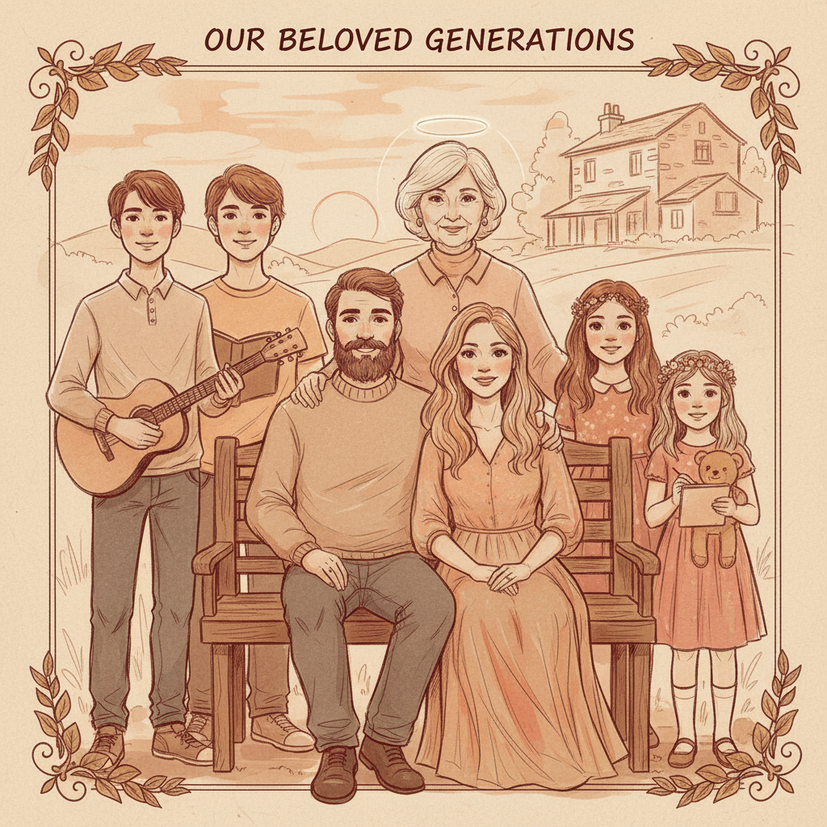
\includegraphics[width=0.85\linewidth]{vokab_300dpi/famill.png} \\
            \vspace{0.3cm}
    }}
    \vspace{0.4em}
    \textbf{\Large D'Famill (Pl. d'Familljen)}\\
    \small\textit{(La famille / The family)}
\end{minipage}
\hfill
\begin{minipage}[t]{0.48\textwidth}
    \centering
    \textbf{\Large E Jong}
    \vspace{0.4em}
    \framebox{\parbox{0.88\linewidth}{\centering
            \vspace{0.3cm}
            
\includegraphics[width=0.85\linewidth]{vokab_300dpi/jong.png} \\
            \vspace{0.3cm}
    }}
    \vspace{0.4em}
    \textbf{\Large De Jong (Pl. d'Jongen)}\\
    \small\textit{(Le garçon / The boy)}
\end{minipage}
\end{noindent}

\vspace{2em}

\begin{noindent}
\begin{minipage}[t]{0.48\textwidth}
    \centering
    \textbf{\Large E Gesiicht}
    \vspace{0.4em}
    \framebox{\parbox{0.88\linewidth}{\centering
            \vspace{0.3cm}
            
\includegraphics[width=0.85\linewidth]{vokab_300dpi/gesicht.png} \\
            \vspace{0.3cm}
    }}
    \vspace{0.4em}
    \textbf{\Large D'Gesiicht (Pl. d'Gesiichter)}\\
    \small\textit{(Le visage / The face)}
\end{minipage}
\hfill
\begin{minipage}[t]{0.48\textwidth}
    \centering
    \textbf{\Large En Auto}
    \vspace{0.4em}
    \framebox{\parbox{0.88\linewidth}{\centering
            \vspace{0.3cm}
            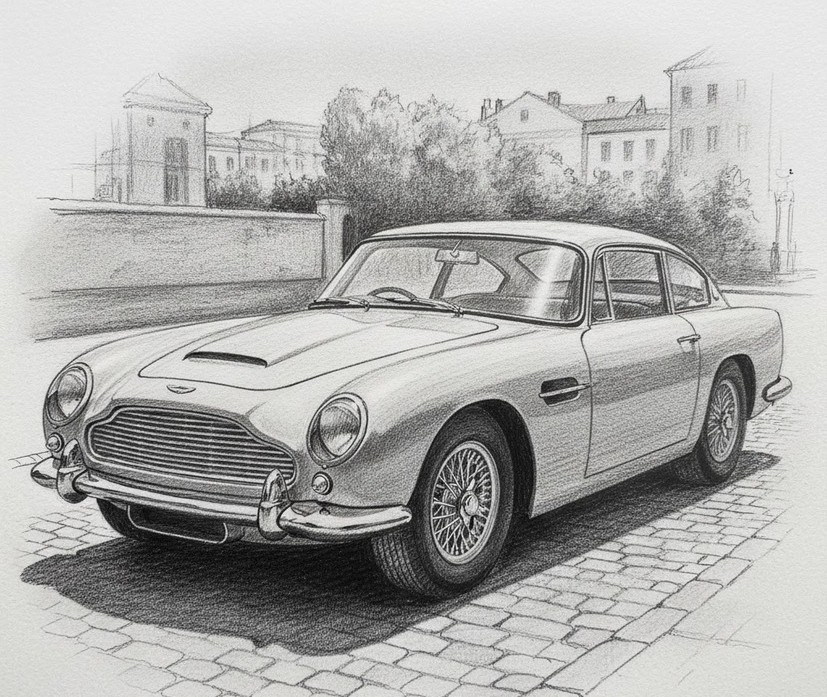
\includegraphics[width=0.85\linewidth]{vokab_300dpi/auto.jpg} \\
            \vspace{0.3cm}
    }}
    \vspace{0.4em}
    \textbf{\Large Den Auto (Pl. d'Autoen)}\\
    \small\textit{(La voiture / The car)}
\end{minipage}
\end{noindent}

\vspace{2em}

\begin{noindent}
\begin{minipage}[t]{0.48\textwidth}
    \centering
    \textbf{\Large En Informatiker}
    \vspace{0.4em}
    \framebox{\parbox{0.88\linewidth}{\centering
            \vspace{0.3cm}
            
\includegraphics[width=0.85\linewidth]{vokab_300dpi/informatiker.png} \\
            \vspace{0.3cm}
    }}
    \vspace{0.4em}
    \textbf{\Large Den Informatiker (Pl. d'Informatiker)}\\
    \small\textit{(L'informaticien / The computer scientist)}
\end{minipage}
\hfill
\begin{minipage}[t]{0.48\textwidth}
    \centering
    \textbf{\Large E Fuerscher}
    \vspace{0.4em}
    \framebox{\parbox{0.88\linewidth}{\centering
            \vspace{0.3cm}
            
\includegraphics[width=0.85\linewidth]{vokab_300dpi/fuerscher.png} \\
            \vspace{0.3cm}
    }}
    \vspace{0.4em}
    \textbf{\Large De Fuerscher (Pl. d'Fuerscher)}\\
    \small\textit{(Le chercheur / The researcher)}
\end{minipage}
\end{noindent}

\vspace{2em}

\begin{noindent}
\begin{minipage}[t]{0.48\textwidth}
    \centering
    \textbf{\Large Eng Blumm}
    \vspace{0.4em}
    \framebox{\parbox{0.88\linewidth}{\centering
            \vspace{0.3cm}
            
\includegraphics[width=0.85\linewidth]{vokab_300dpi/blumm.png} \\
            \vspace{0.3cm}
    }}
    \vspace{0.4em}
    \textbf{\Large D'Blumm (Pl. d'Blummen)}\\
    \small\textit{(La fleur / The flower)}
\end{minipage}
\hfill
\begin{minipage}[t]{0.48\textwidth}
    \centering
    \textbf{\Large Geméis}
    \vspace{0.4em}
    \framebox{\parbox{0.88\linewidth}{\centering
            \vspace{0.3cm}
            
\includegraphics[width=0.85\linewidth]{vokab_300dpi/gemies.png} \\
            \vspace{0.3cm}
    }}
    \vspace{0.4em}
    \textbf{\Large D'Geméis}\\
    \small\textit{(Les légumes / The vegetables)}
\end{minipage}
\end{noindent}
